% #############################################################################
\begin{frame}[standout]

    \alert{Uma palavra que associem à Inteligência Artificial (IA)?}
    
    \tiny{Vamos começar com uma \textit{chuva de ideias}!}
    
    %% Notes:
    \note{-- É uma invenção humana que permite simular comportamentos humanos inteligentes.
    -- Existem agentes (e.g., robôs) que recebem as informações do meio, raciocinam e agem.
    -- É uma combinação de diferentes áreas e a computação.
    }

\end{frame}
% #############################################################################

% #############################################################################
\section*{Motivação}
% #############################################################################

% #############################################################################
\begin{frame}[standout]
    
    O que é uma \textit{porta}?
    
    \tiny{Não se refira ao termo informático de \textit{porta}.}
    
    \medskip
    
    \begin{columns}
        \begin{column}{0.3\textwidth}
            \includegraphics<2->[width=\textwidth]{doors/door1}
        \end{column}
        \begin{column}{0.3\textwidth}
            \includegraphics<3->[width=\textwidth]{doors/door2}
        \end{column}
        \begin{column}{0.3\textwidth}
            \includegraphics<4->[width=\textwidth]{doors/door3}
        \end{column}
    \end{columns}

\end{frame}
% #############################################################################

% #############################################################################
\begin{frame}[fragile]{Motivação}

    Vamos \textbf{desenvolver um algoritmo} para detectar o objecto \textit{porta}.

    \pauseskip

    \begin{lstlisting}[language=Python]
def is_door(object):
    if object.has_handle():
        if object.has_keyhole():
            if object.shape == 'cuboid':
                if object.height >= 2 and object.width >= 0.8:
                    return True
    return False\end{lstlisting}
    
    \pausenormal
    \vspace{-.5cm}
    
    Este algoritmo segue o paradigma da \alertbf{programação tradicional}\footnote{Mais concretamente, o paradigma da programação imperativa.}:
    
    \begin{figure}
        \centering
        \begin{tikzpicture}[node distance=2cm]
    \node (input) at (0,0) [circle_s] {\textit{Inputs}};
    \node (regra) [circle_s, right of=input, align=center, xshift=1.5cm] {Regras};
    \node (output) [circle_important, right of=regra, align=center, xshift=1.5cm] {\textit{Output}};
    \draw [arrow] (input) -- (regra);
    \draw [arrow] (regra) -- (output);
\end{tikzpicture}
    \end{figure}
            
\end{frame}
% #############################################################################

% #############################################################################
\begin{frame}[standout]
    
    Vejamos outros exemplos de portas\ldots
    
    \bigskip
    
    \begin{columns}
        \begin{column}{0.3\textwidth}
            \includegraphics<2->[width=\textwidth]{doors/door4}
        \end{column}
        \begin{column}{0.3\textwidth}
            \includegraphics<3->[width=\textwidth]{doors/door5}
        \end{column}
        \begin{column}{0.3\textwidth}
            \includegraphics<4->[width=\textwidth]{doors/door6}
        \end{column}
    \end{columns}

\end{frame}
% #############################################################################

% #############################################################################
\begin{frame}{Motivação \cont}

    Nesses exemplos, o nosso algoritmo \textbf{não vai retornar a resposta correcta}.

    \pausenormal

     Vamos a \textbf{mais um exemplo}. Conseguiremos predizer, como base na temperatura, na humidade e no vento, se iremos ter condições favoráveis à prática de ténis\footnote{Exemplo adaptado de:  Oliveira, A., 2017. Mentes Digitais. A Ciência Redefinindo a Humanidade.}?

  \begin{table}
    \begin{tabular}{SSS|c}
      \toprule
      {Temp. (\SI{}{\degreeCelsius})} & {Humidade (\SI{}{\percent})} & {Vento (\SI{}{\kilo\metre\per\hour})} & {Jogar ténis?} \\
      \midrule
      21 & 95 &  5 & \textbf{Sim} \\
      0  & 80 & 10 & \alertbf{Não} \\
      24 & 85 & 10 & \textbf{Sim} \\
      18 & 80 & 20 & \alertbf{Não} \\
      15 & 35 &  8 & \textbf{Sim} \\
      -1 & 35 &  8 & \alertbf{Não} \\
      22 & 35 & 25 & \textbf{Sim} \\
      \bottomrule
    \end{tabular}
  \end{table}

  %% Notes:  
  \note{-- Identificar os inputs e os outputs.
  -- Identificar a necessidade de fazer feature selection. A variável Humidade não é necessária.
  -- Identificar que nem sempre conseguimos encontrar a regras que satisfaçam tudo... temos de encontrar as regras que minizem o número de casos identificados erradamente.}
  
\end{frame}
% #############################################################################

% #############################################################################
\begin{frame}{Motivação \cont}
    \tikzstyle{process} = [rectangle, minimum width=1.5cm, minimum height=1cm, text centered, draw=black, fill=TolLightRed]
    \tikzstyle{process_yes} = [rectangle, minimum width=1.5cm, minimum height=1cm, text centered, draw=black, fill=TolLightGreen]
    \tikzstyle{decision} = [diamond, minimum width=3cm, minimum height=1cm, text centered, draw=black, fill=TolLightBlue]
    \tikzstyle{arrow} = [thick,->,>=stealth]

    Vamos criar (um possível) \textbf{conjunto de regras}\ldots

    \begin{figure}
        \centering
        \begin{tikzpicture}[node distance=2cm]
            \node (temp) [decision] {Temp.?};
            \node (vento) [decision, below of=temp, xshift=3cm] {Vento?};
            \node (nao_temp) [process, left of=vento, xshift=-4cm] {Não};
            \node (sim) [process_yes, below of=vento, xshift=3cm] {Sim};
            \node (nao_vento) [process, left of=sim, xshift=-4cm] {Não};
            \draw [arrow] (temp) -| node[anchor=south] {$\ge$ \SI{10}{\degreeCelsius}} (vento);
            \draw [arrow] (temp) -| node[anchor=south] {$<$ \SI{10}{\degreeCelsius}} (nao_temp);        
            \draw [arrow] (vento) -| node[anchor=south] {$\le$ \SI{15}{\kilo\metre\per\hour}} (sim);
            \draw [arrow] (vento) -| node[anchor=south] {$>$ \SI{15}{\kilo\metre\per\hour}} (nao_vento);
        \end{tikzpicture}
    \end{figure}
    
\end{frame}
% #############################################################################

% #############################################################################
\begin{frame}{Motivação \cont}

    Neste exemplo, usámos \textbf{dois tipos de raciocínio}:

    \bigskip

    \begin{columns}[T,onlytextwidth]
    \column{0.45\textwidth}
      
      \metroset{block=fill}
      \begin{block}{Indutivo}
        Usa a experiência anterior para \alert{determinar o caso geral}.
      \end{block}
       
       \medskip
       
      \scriptsize{O exame de Física correu bem.}\\
      \scriptsize{O exame de Matemática correu bem.}\\
      \scriptsize{O exame de Química correu bem.}\\
      \scriptsize{Os exames foram feitos em Quartas-feiras.}\\
      \scriptsize{Logo, todos os testes feitos às Quartas-feiras correm bem.}

    \column{0.50\textwidth}

      \metroset{block=fill}
      \begin{block}{Dedutivo}
        Usa o caso geral para \alert{determinar casos específicos}.
      \end{block}

      \medskip
      
      \scriptsize{Todos os homens são mortais.}\\
      \scriptsize{Sócrates é homem.}\\
      \scriptsize{Logo, Sócrates é mortal.}
      
  \end{columns}

\end{frame}
% #############################################################################

% #############################################################################
\begin{frame}{Motivação \cont}

    \alertbf{Criar conjuntos de regras \textit{manualmente} é complicado. Como podemos, então, criar conjuntos de regras de forma automática?}

    \pauseskip

    Uma solução passa por utilizar \alertbf{aprendizagem automática}:
    \begin{figure}
        \centering
        \begin{tikzpicture}[node distance=2cm]
    \node (input) at (0,0) [circle_s] {\textit{Inputs}};
    \node (output) [circle_s, right of=input, align=center, xshift=1.5cm] {\textit{Output}};
    \node (regra) [circle_important, right of=output, align=center, xshift=1.5cm] {Regras};
    \draw [arrow] (input) -- (output);
    \draw [arrow] (output) -- (regra);
\end{tikzpicture}
    \end{figure}
    
    \pauseskip
    
    Permite um sistema \textbf{aprender com a experiência} (indutivo), \textit{i.e.}, o \textbf{sistema escreve automaticamente as regras} para os casos gerais (dedutivo).

    \pauseskip
   
    As \alertbf{redes neuronais artificiais} podem ser usadas para \textbf{atingir a aprendizagem automática} de um sistema. 
    
\end{frame}
% #############################################################################


% #############################################################################
\begin{frame}{Agenda}
  \setbeamertemplate{section in toc}[sections numbered]
  \tableofcontents%[hideallsubsections]
\end{frame}
% #############################################################################

% #############################################################################
\section{Introdução}
% #############################################################################

% #############################################################################
\begin{frame}{Introdução}

    \alertbf{Onde estamos no panorama da IA?}
    
    \medskip

    \begin{figure}
			\centering
			\resizebox{!}{0.5\linewidth}{
				\smartdiagram[bubble diagram]{Inteligência\\ Artificial,
  Robótica, Processamento de\\ linguagem natural, Sistemas\\ especialistas, \ldots, Aprendizagem\\ automática}
			}
	\end{figure}

    \medskip

    A IA foi motivada pela automação de processos e resultou na Aprendizagem Automática, que corresponde à extracção de conhecimento a partir de dados.
	
\end{frame}
% #############################################################################

% #############################################################################
\begin{frame}{Introdução \cont}
		    
	As \textbf{Redes Neuronais Artificiais (RNAs)} foram criadas para \textbf{permitir que as máquinas} se comportem como \textbf{agentes inteligentes}.
		    
	\medskip
		    
	Elas \textit{imitam} a forma de como os nossos \textbf{neurónios se interconectam}, bem como \textbf{forma de como nós aprendemos}---\alertbf{inferência indutiva}.
	
	\medskip
	
	\begin{figure}
		\centering
		\begin{subfigure}{0.45\textwidth}
			\centering
			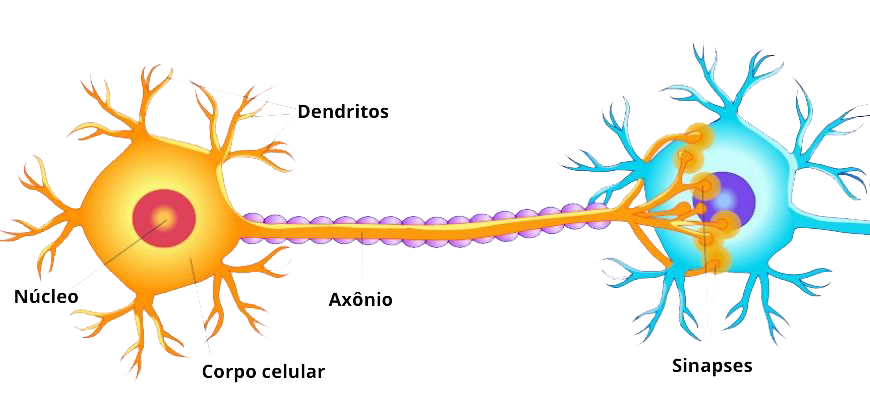
\includegraphics[width=\linewidth]{Biological}
		\end{subfigure}
		\begin{subfigure}{0.45\textwidth}
			\centering
			\resizebox{!}{0.7\linewidth}{
				\begin{tikzpicture}[shorten >=1pt,->, node distance=\layersep]
    \tikzstyle{every pin edge}=[<-,shorten <=2pt]
    \tikzstyle{neuron}=[circle,draw,minimum size=25pt,inner sep=0pt]
    \tikzstyle{output neuron}=[draw,minimum size=25pt, minimum width=50pt,inner sep=0pt]
    \tikzstyle{input neuron}=[neuron];
    \tikzstyle{hidden neuron}=[neuron];
    \tikzstyle{annot} = [text centered]

    % Draw the input layer nodes
    \node[input neuron] (I-1) at (0,-1) {$i_{1}$};
    \node[input neuron] (I-2) at (0,-2.2) {$i_{2}$};
    \node (I-etc) at (0,-3) {$\vdots$};
    \node[input neuron] (I-3) at (0,-4) {$i_j$};

    % Draw the hidden layer nodes
    \node[output neuron ,pin={[pin edge={->}]right:Axónio}] (H-1) at (\layersep,-2.5 cm) {Neurónio};

    % Connect every node in the input layer with every node in the
    % hidden layer.
    \path (I-1) edge node[above]{$w_{1}$} (H-1);
    \path (I-2) edge node[above]{$w_{2}$} (H-1);
    \path (I-3) edge node[above, xshift=-0.2cm]{$w_j$} (H-1);
    
    % Annotate the layers
    \node[annot,above of=I-3, yshift=-3.5cm] (hl) {Dendrites com sinapses};
\end{tikzpicture}

			}
		\end{subfigure}
		\caption{Rede neuronal biológica (esquerda) e rede neuronal artificial (direita).}
	\end{figure}
		    
	%% Notes:
	\note{ -- Para permitir que as máquinas respondam a situações para as quais ela \alertbf{não fora programada para tal}.
	
	       -- \alertbf{Explicar as conexões:} Os neurónios são conectados uns aos outros com o uso de axónios e dentritos, e as regiões de conexão entre os axónios e dentritos são chamadas de sinapses.
	       
	       -- A importância de cada conexão sináptica muda em resposta a estímulos externos, e é \alertbf{assim que aprendemos}. 
	       
	       -- Esta é uma \alertbf{caracterização muito simplista} da forma de como os nossos neurónios funcionam. Mas dá, apesar das críticas, para ter uma ideia deste paralelo. 
        }
		    
\end{frame}
% #############################################################################

% #############################################################################
\begin{frame}{Introdução \cont}
		
	\textbf{McCulloch e Pitts} são considerados os \textit{pais} das RNAs. 
		    
	De acordo com estes autores, os neurónios faziam \textbf{uma soma ponderada ($\mathbf{w}$) das suas entradas ($\mathbf{i}$)} para implementar qualquer função lógica.
		   
	\pauseskip
		
	Nos finais dos anos 50 e começo dos anos 60, \textbf{Rosenblatt introduziu o perceptrão}.
		    
	Os perceptrões faziam uma \textbf{soma ponderada} das suas entradas, mas o \textbf{\textit{output} ($\hat{y}$) era binário}, de tal forma que:
	\begin{equation}
		\hat{y} = \begin{cases}
		0, \; \text{se} \; \sum_j w_j i_j \leq \text{limiar}, \\
		1, \; \text{caso contrário}.
		\end{cases}
	\end{equation}
		    
	%% Notes:
	\note{-- Em \alertbf{1943}, McCulloch e Pitts desenvolveram o primeiro modelo computacional para a RNA utilizando um \alertbf{modelo linear}.

         -- Este trabalho é considerado o \alertbf{primeiro modelo computacional} que pode aprender como \alertbf{ajustar os pesos sinápticos}, a fim de classificar as entradas \alertbf{em duas categorias, com base em exemplos dados anteriormente (ou seja, supervised learning)}.
	}
		    
\end{frame}
% #############################################################################

% #############################################################################
\begin{frame}{Introdução \cont}
		    
	\begin{example}[Calcular o \textit{output} de um perceptrão:]
		\label{exmp:andgate}
		\medskip
		\begin{minipage}{0.45\linewidth}
			\begin{figure}
				\centering
				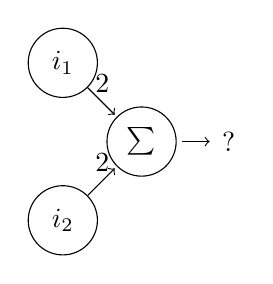
\begin{tikzpicture}[shorten >=1pt,->, node distance=\layersep]
    \tikzstyle{every pin edge}=[<-,shorten <=2pt]
    \tikzstyle{neuron}=[circle,draw,minimum size=25pt,inner sep=0pt]
    \tikzstyle{output neuron}=[draw,minimum size=25pt, minimum width=50pt,inner sep=0pt]
    \tikzstyle{input neuron}=[neuron];
    \tikzstyle{hidden neuron}=[neuron];
    \tikzstyle{annot} = [text centered]

    % Draw the input layer nodes
    \node[input neuron] (I-1) at (0,1) {$i_{1}$};
    \node[input neuron] (I-2) at (0,-1) {$i_{2}$};

    % Draw the hidden layer nodes
    \node[neuron ,pin={[pin edge={->}]right:?}] (H-1) at (\layersep,0) {$\sum$};

    % Connect every node in the input layer with every node in the
    % hidden layer.
    \path (I-1) edge node[above]{2} (H-1);
    \path (I-2) edge node[above]{2} (H-1);

\end{tikzpicture}

			\end{figure}
			\alertbf{Segundo caso:} $i_1 = 1$ e $i_2 = 0$, obtemos $2$.
						
			\alertbf{Terceiro caso:} $i_1 = 0$ e $i_2 = 1$, obtemos $2$.
						
			\alertbf{Quarto caso:} $i_1 = i_2 = 0$, obtemos $0$.
		\end{minipage}
		\begin{minipage}{0.45\linewidth}
			\alertbf{Primeiro caso:} $i_1 = i_2 = 1$
			\begin{equation}
				\begin{split}
					\sum_{j=1}^{2} w_j i_j &= w_1 i_1 + w_2 i_2 \\ 
					&= 2 \times 1 + 2 \times 1 = 4.
				\end{split}
			\end{equation}
			\textbf{Se considerarmos um limiar de 2, os \textit{outputs} vêm:}
			\begin{table}
				\centering
				\begin{tabular}{c|ccc}
					\toprule
					Caso & $i_1$ & $i_2$ & \textit{Output} \\
					\midrule
					1    & 1     & 1     & 1               \\
					2    & 1     & 0     & 0               \\
					3    & 0     & 1     & 0               \\
					4    & 0     & 0     & 0               \\
					\bottomrule
				\end{tabular}
			\end{table}
		\end{minipage}
	\end{example}
	
	%% Notes:
	\note{-- Neste exemplo, podemos verificar que o perceptrão consegue \alertbf{modelar o resultado lógico de uma porta AND}.
	
	      -- Assim, mostramos que um perpetração consegue modelar \alertbf{funções lógicas (pelo menos as mais simples) -- incluindo as operações lógicas da \alertbf{máquina de Turing}.}.
	      
	      -- As funções lógicas \alertbf{mais complexas podem ser modelas interconectando perceptrões}.
    	}
		
\end{frame}
% #############################################################################

% #############################################################################
\begin{frame}{Introdução \cont}
		
	Vamos, agora, \textbf{alterar um pouco a notação}, e considerar $b = -\text{limiar}$. Desta forma, o \textit{output} de um perceptrão vem:
	\begin{equation}
		\label{eq:outputbias}
		\hat{y} = \begin{cases}
		0, \; \text{se} \; \sum_j w_j i_j + b \leq 0, \\
		1, \; \text{caso contrário}.
		\end{cases}
	\end{equation}
		    
	\alertbf{O termo $b$ é conhecido como \textit{bias}.}
		    
	\pauseskip
		
	Se considerarmos $\mathbf{W} = \left [ w_1, w_2, \cdots, w_j \right ]$ e $\mathbf{I} = \left [ i_1, i_2, \cdots, i_j \right ]$, a Equação \eqref{eq:outputbias} pode ser reescrita, de tal forma que:
	\begin{equation}
		\hat{y} = \begin{cases}
		0, \; \text{se} \; \mathbf{W} \cdot \mathbf{I} + b \leq 0, \\
		1, \; \text{caso contrário},
		\end{cases}
	\end{equation}
	onde $\cdot$ denota o produto interno.
		
	%%  Notes:
	\note{ -- Podemos pensar que o bias é uma \alertbf{medida de quão fácil é fazer o percepção disparar}. 
	
	       -- Se o bias for \alertbf{extremamente alto, o perceptrão disparará mais facilmente}.  
	    }
		
\end{frame}
% #############################################################################

% #############################################################################
\begin{frame}{Introdução \cont}
		
	\begin{figure}
		\centering
		\begin{subfigure}{0.45\textwidth}
			\centering
			\resizebox{!}{0.7\linewidth}{
				\begin{tikzpicture}
\begin{axis}[ticks=none]
\addplot[domain=0:10, TolDarkBrown] {1.4323*x + 0.4495};
\addplot[only marks, TolLightRed] coordinates {(0, 2.41) (1, 3.55) (6, 14.97) (7, 11.89) (8, 14.65)};
\addplot[only marks, TolLightGreen] coordinates {(2, 1.54) (3, 1.65) (4, 4.28) (5, 3.96) (9, 10.80) (10, 14.02)};
\end{axis}
\end{tikzpicture}
			}
		\end{subfigure}
		\begin{subfigure}{0.45\textwidth}
			\centering
			\resizebox{!}{0.7\linewidth}{
				\begin{tikzpicture}
\begin{axis}[ticks=none]
\addplot3[domain=0:1, TolDarkBrown] {(-2)*x + (-2)*y + 3};
\addplot3[only marks, TolLightRed] coordinates {(0, 0, 0) (1, 0, 0)};
\addplot3[only marks, TolDarkRed] coordinates {(0, 1, 0)};
\addplot3[only marks, TolLightGreen] coordinates {(1, 1, 1)};
\end{axis}
\end{tikzpicture}
			}
		\end{subfigure}
		\caption{Recta (esquerda) e plano (direita) de regressão que se podem obter de um perceptrão.}
	\end{figure}
		    
	Contudo, nós só \textbf{sabemos as entradas} e os \textit{\textbf{outputs}} esperados.
    
    \pauseskip
    
	É necessário \textbf{ajustar automaticamente os pesos e os \textit{bias} de um perceptrão}---\alertbf{algoritmos de aprendizagem}.
		    
\end{frame}
% #############################################################################

% #############################################################################
\begin{frame}{Introdução \cont}
		
	\begin{figure}
		\centering
		\resizebox{!}{0.4\textwidth}{
			\begin{tikzpicture}
\begin{axis}[ticks=none, domain=0:10]
\addplot[TolDarkRed] {1.5*x};
\addplot[TolDarkGreen] {2*x};
\draw [thick,decoration={brace,mirror,raise=5pt},decorate,visible on=<2->] (axis cs:8,12.5) -- node[right=7pt] {$E$} (axis cs:8,16.5);
\draw [<-] (axis cs:8.3,17)-- +(0pt, 15pt) node[left] {Valor esperado~($y$)};
\draw [->] (axis cs:8.3,5)-- +(0pt, 45pt) node[below=50pt] {Valor calculado~($\hat{y}$)};
\end{axis}
\end{tikzpicture}
		}
		\caption{Visualização gráfica do cálculo do erro ($E$).}
	\end{figure}
		    
	O erro ($E$) é dado por $E = y - \hat{y}$.
	
	\pauseskip
	
	Este \textbf{erro é depois usado pelo algoritmo de aprendizagem} para ajustar a linha de modo a \alertbf{minimizar} o erro. 
		
\end{frame}
% #############################################################################

% #############################################################################
\begin{frame}{Introdução \cont}
		    
	Podemos escrever o \textit{output} do percepção da seguinte forma:
	\begin{equation}
		\mathbf{y} = (\mathbf{W} + \Delta \mathbf{W}) \cdot \mathbf{I},
	\end{equation}
	onde $\Delta$ denota um factor de mudança.
	
	\pauseskip
	
	Assim, 
	\begin{equation}
		\begin{split}
			\mathbf{E} &= \mathbf{y} - \hat{\mathbf{y}} \\
			&= (\mathbf{W} + \Delta \mathbf{W}) \cdot \mathbf{I} - \mathbf{W} \cdot \mathbf{I} \\
			&= (\Delta \mathbf{W}) \cdot \mathbf{I},
		\end{split}
	\end{equation}
	e, desta forma, 
	\begin{equation}
		\Delta \mathbf{W} = \frac{\mathbf{E}}{\mathbf{I}}.
	\end{equation}
		
	\pauseskip
	
	Contudo, o mais comum é considerar a seguinte equação, onde $\alpha$ é conhecido como \alertbf{\textit{learning rate}} (ou \textbf{tamanho do passo}):
	\begin{equation}
		\Delta \mathbf{W} = \alpha \left(\frac{\mathbf{E}}{\mathbf{I}} \right).
	\end{equation}
		
	%% Notes:
	\note{ -- Mas nós temos um problema: sempre que usamos um exemplo para treinar a rede, estamos a actualizar os \alertbf{pesos totalmente consoante o erro desse exemplo}.
	
	       -- Desta forma, em vez de ter usado os exemplos todos, usava só o exemplo final e actual os pesos consoante isso. 
	       
	       -- O que fazemos é considerar \alertbf{sempre uma porção de actualização. Mantemos a direcção mas moderamos a mudança}.
	       
		    -- \alertbf{O bias pode ser colocado sempre a UM e ter um peso associado}. Assim, ao optimizar os pesos das ligações estamos, também, a optimizar o peso do bias.
	}
		
\end{frame}
% #############################################################################

% #############################################################################
\begin{frame}{Introdução \cont}
	    
	Quando foram propostos, os \textbf{perceptrões despertaram um interesse significativo na comunidade científica}. Isto porque:
	\begin{itemize}
		\item Eram muito \textbf{semelhantes aos neurónios reais}, que só disparam quando a quantidade de excitação é alta;
		\medskip
		\item Existia um \textbf{algoritmo de aprendizagem simples} para ajustar os pesos. 
	\end{itemize}
	    
	\pauseskip 
	
	Contudo, os perceptrões só poderiam ser usados em \textbf{problemas linearmente separáveis}, uma vez que a \textbf{soma ponderada é uma função linear}. 
	    
	%% Notes: 
	\note{ -- Os perceptrões eram conhecidos como o \alertbf{embrião de um computador}.
	
	       -- \alertbf{Problemas linearmente} separáveis quer dizer que as instâncias negativas podem ser separadas das instâncias positivas por uma linha recta.
	}
	
\end{frame}
% #############################################################################

% #############################################################################
\begin{frame}{Introdução \cont}
	    
	Para exemplificar esta limitação, vejamos, agora, \alertbf{a porta lógica XOR}:
	    
	\medskip
	
	\begin{minipage}{0.45\linewidth}
		\begin{table}
			\centering
			\begin{tabular}{ccc}
				\toprule
				$i_1$ & $i_2$ & \textit{Output} \\
				\midrule
				1     & 1     & 0               \\
				1     & 0     & 1               \\
				0     & 1     & 1               \\
				0     & 0     & 0               \\
				\bottomrule
			\end{tabular}
		\end{table}
	\end{minipage}
	\begin{minipage}{0.45\linewidth}
		\begin{figure}
			\centering
			\resizebox{!}{0.7\textwidth}{
				\begin{tikzpicture}
\begin{axis}[ticks=none, xmin=-1.5, xmax=1.5, ymin=-1.5, ymax=1.5,
axis line style={shorten >=-10pt, shorten <=-10pt},
axis y line=center,
axis x line=middle,
no markers]

\addplot[only marks, TolLightGreen] coordinates {(-1, 1) (1, -1)};
\addplot[only marks, TolLightRed] coordinates {(1, 1) (-1, -1)};

\node[] at (axis cs: -1, 1.2) {(0, 1)};
\node[] at (axis cs: -1, -0.8) {(0, 0)};
\node[] at (axis cs: 1, 1.2) {(1, 1)};
\node[] at (axis cs: 1, -0.8) {(1, 0)};

\addplot[color=TolDarkBlue, visible on=<2>]{x+0.5};
\addplot[color=TolLightBrown, visible on=<3>]{-x+0.5};
\addplot[color=TolLightGreen, visible on=<4>]coordinates {(0.8,1.5)(0.8,-1.5)};
\addplot[color=TolDarkPink, visible on=<5>]coordinates {(-0.8,1.5)(-0.8,-1.5)};

\end{axis}
\end{tikzpicture}
			}
		\end{figure}
	\end{minipage}
    
    \medskip
    
	\only<5>{
	Por esta razão, \textbf{surgem as RNAs} como \textbf{modelos computacionais que resultam da conexão de neurónios simples}.
	}
	
\end{frame}
% #############################################################################

% #############################################################################
\section{Redes Neuronais Artificiais}
% #############################################################################

% #############################################################################
\begin{frame}{Redes Neuronais Artificiais}

\metroset{block=fill}
\begin{exampleblock}{O que são \textit{features}?}
    \textit{Features} ou \textit{atributos} são propriedades que \textbf{descrevem uma possível relação com a variável de saída}. Os atributos podem ser numéricos ou categóricos.
    
    \textbf{\textit{E.g.}}, altura e temperatura.
\end{exampleblock}

\pauseskip

\begin{columns}
    \begin{column}{0.45\textwidth}
        \metroset{block=fill}
        \begin{alertblock}{Criação de \textit{features}}
            Métodos manuais ou automáticos de \textbf{criação de novos atributos com base nos que já existem}.
        \end{alertblock}
    \end{column}
    \pause
    \begin{column}{0.45\textwidth}
        \metroset{block=fill}
        \begin{block}{Selecção de \textit{features}}
            Métodos manuais ou automáticos para \textbf{reduzir a dimensionalidade do problema}.
        \end{block}
    \end{column}
\end{columns}

%% Notes:
\note{-- os atributos são normalmente considerados como variáveis dependentes, ou seja, o X--input dos modelos. A variável independente é o Y.
      -- Dar exemplos. Estimar o peso (idade, altura, tamanho do calçado).
      -- Selecção de feautures permite reduzir o número de entradas)}

\end{frame}
% #############################################################################

% #############################################################################
\begin{frame}{Redes Neuronais Artificiais \cont}
	
	\begin{figure}
		\centering
		\resizebox{!}{0.4\textwidth}{
			\begin{tikzpicture}[shorten >=1pt,->,draw=black, node distance=\layersep]
    \tikzstyle{every pin edge}=[<-,shorten <=1pt]
    \tikzstyle{neuron}=[circle,minimum size=17pt, draw=black, inner sep=0pt]
    \tikzstyle{input neuron}=[neuron];
    \tikzstyle{output neuron}=[neuron];
    \tikzstyle{hidden neuron}=[neuron];
    \tikzstyle{annot} = [text width=5em, text centered]

    % Draw the input layer nodes
    \foreach \name / \y in {1,...,4}
    % This is the same as writing \foreach \name / \y in {1/1,2/2,3/3,4/4}
        \node[input neuron] (I-\name) at (0,-\y) {$i_{\y}$};

    % Draw the hidden layer nodes
    \foreach \name / \y in {1,...,5}
        \path[yshift=0.5cm]
            node[hidden neuron] (H-\name) at (\layersep,-\y cm) {};

    % Draw the output layer node
    \node[output neuron,pin={[pin edge={->}]right:$\hat{y}$}, right of=H-3] (O) {};

    % Connect every node in the input layer with every node in the
    % hidden layer.
    \foreach \source in {1,...,4}
        \foreach \dest in {1,...,5}
            \path (I-\source) edge (H-\dest);

    % Connect every node in the hidden layer with the output layer
    \foreach \source in {1,...,5}
        \path (H-\source) edge (O);

    % Annotate the layers
    \node[annot,above of=H-1, node distance=1cm] (hl) {Camada oculta};
    \node[annot,left of=hl] {Camada de entrada (\textit{features})};
    \node[annot,right of=hl] {Camada de saída};
\end{tikzpicture}

		}
		\caption{Arquitectura de uma rede neuronal artificial.}
	\end{figure}
	    
	Numa RNA, os neurónios \textbf{não têm um limiar rígido, mas gradual}.
    
    \pauseskip
    
	Isso significa que \textbf{pequenas mudanças nas entradas ou nos pesos de conexão levam a pequenas mudanças na saída}. 
	    
	%% Notes:
	\note{-- Explicar as camadas, e profundidade.
		    
		-- Numa RNA, os perceptrões não têm um limiar rígido, mas gradual, o que veio a facilitar o desenvolvimento de algoritmos de aprendizagem eficientes. 
		    
		-- Estes algoritmos de aprendizagem irão, em princípio, derivar os pesos óptimos para uma RNA arbitrária.
		    
		-- Cada neurónio calcula uma função que é suave e matematicamente bem comportada. 
	}
	
\end{frame}
% #############################################################################

% #############################################################################
\begin{frame}{Redes Neuronais Artificiais \cont}
	
	\begin{figure}
		\centering
		\resizebox{!}{0.4\textwidth}{
			\begin{tikzpicture}[shorten >=1pt,->, node distance=\layersep]
    \tikzstyle{every pin edge}=[<-,shorten <=2pt]
    \tikzstyle{neuron}=[circle,draw,minimum size=25pt,inner sep=0pt]
    \tikzstyle{output neuron}=[draw,minimum size=25pt,inner sep=0pt]
    \tikzstyle{input neuron}=[neuron];
    \tikzstyle{hidden neuron}=[neuron];
    \tikzstyle{annot} = [text width=5em, text centered]

    % Draw the input layer nodes
    \node[input neuron] (I-1) at (0,-1) {$i_{1}$};
    \node[input neuron] (I-2) at (0,-2.5) {$i_{2}$};
    \node (I-etc) at (0,-3.5) {$\vdots$};
    \node[input neuron] (I-3) at (0,-4.7) {$i_{j}$};


    % Draw the hidden layer nodes
    \foreach \name / \y in {1,...,1}
        \path[yshift=0.cm]
            node[hidden neuron] (H-\name) at (\layersep,-2.5 cm) {$\sum$};

    % Draw the output layer node
    \node[output neuron,pin={[pin edge={->}]right:Saída}, right of=H-1] (O) {$\phi$};

    % Connect every node in the input layer with every node in the
    % hidden layer.
    \path (I-1) edge node[above]{$w_{1}$} (H-1);
    \path (I-2) edge node[above]{$w_{2}$} (H-1);
    \path (I-3) edge node[above]{$w_{j}$} (H-1);
    
    % Connect every node in the hidden layer with the output layer
    \foreach \source in {1,...,1}
        \path (H-\source) edge (O);

    % Annotate the layers
    \node[annot,above of=H-1, node distance=2.5cm] (hl) {Soma ponderada};
    \node[annot,left of=hl] {Entrada};
    \node[annot,right of=hl] {Função de activação};
\end{tikzpicture}
		}
		\caption{Arquitectura de um neurónio de uma RNA.}
	\end{figure}
	    
	Os neurónios numa \textbf{RNA têm duas funções}: 
	\begin{itemize}
		\item \textbf{Função de transferência} ($\mathbf{T} = \mathbf{W} \cdot \mathbf{I}$);
		\item \textbf{Função de activação} ($\phi$).
	\end{itemize}
	    
	%% Notes:
	\note{-- Essa saída será então transmitida para o neurónio seguinte da próxima camada, até a camada de saída. Este processo de transmissão é conhecido como forward propagation.}
	
\end{frame}
% #############################################################################

% #############################################################################
\begin{frame}{Redes Neuronais Artificiais \cont}
	
	Assim, a saída de um neurónio é calculada da seguinte forma:
	\begin{equation}
		O_j = \phi(T_j).
	\end{equation}
	    
	\begin{figure}
		\centering
		\begin{subfigure}{0.45\textwidth}
			\centering
			\resizebox{!}{0.4\linewidth}{
				\begin{tikzpicture}
\begin{axis}[
axis line style={shorten >=-10pt, shorten <=-10pt},
axis y line=center,
axis x line=middle,]
\addplot[domain=-5:5, TolDarkBrown] {1/(1+e^(-x)};
\end{axis}
\end{tikzpicture}
			}
			\caption{Sigmóide.}
		\end{subfigure}
		\medskip
		\begin{subfigure}{0.45\textwidth}
			\centering
			\resizebox{!}{0.4\linewidth}{
				\begin{tikzpicture}
\begin{axis}[
axis line style={shorten >=-10pt, shorten <=-10pt},
axis y line=center,
axis x line=middle,]
\addplot[domain=-5:5, TolDarkBrown] {tanh(x)};
\end{axis}
\end{tikzpicture}
			}
			\caption{Tangente hiperbólica.}
		\end{subfigure}
		\medskip
		\begin{subfigure}{0.45\textwidth}
			\centering
			\resizebox{!}{0.4\linewidth}{
				\begin{tikzpicture}
\begin{axis}[
axis line style={shorten >=-10pt, shorten <=-10pt},
axis y line=center,
axis x line=middle,]
\addplot+[mark=none,TolDarkBrown,domain=-5:0] {0};
\addplot+[mark=none,TolDarkBrown,domain=0:5] {x};
\end{axis}
\end{tikzpicture}
			}
			\caption{Unidade Linear Retificada (ReLU).}
		\end{subfigure}
		\begin{subfigure}{0.45\textwidth}
			\centering
			\resizebox{!}{0.4\linewidth}{
				\begin{tikzpicture}
\begin{axis}[
axis line style={shorten >=-10pt, shorten <=-10pt},
axis y line=center,
axis x line=middle,]
\addplot[domain=-5:5, TolDarkBrown] {x};
\end{axis}
\end{tikzpicture}
			}
			\caption{Identidade.}
		\end{subfigure}
		\caption{Exemplos de funções de activação.}
	\end{figure}
	
	%% Notes:
	\note{-- Poderão verificar que maior parte das funções de activação são não lineares. Isto permite que as redes aprendam relações não-lineares entre as variáveis de entrada e a saída.}
	
\end{frame}
% #############################################################################

% #############################################################################
\section{\textit{Forward Propagation}}
% #############################################################################

% #############################################################################
\begin{frame}{\textit{Forward Propagation}}
	
	Agora que já sabemos a função de cada neurónio na rede, vamos estudar o conceito de \alertbf{\textit{forward propagation}}.
	    
	\begin{figure}
		\centering
		\begin{tikzpicture}[shorten >=1pt,->,draw=black, node distance=\layersep]
    \tikzstyle{every pin edge}=[<-,shorten <=1pt]
    \tikzstyle{neuron}=[circle,minimum size=17pt, draw=black, inner sep=0pt]
    \tikzstyle{input neuron}=[neuron];
    \tikzstyle{output neuron}=[neuron];
    \tikzstyle{hidden neuron}=[neuron];
    \tikzstyle{annot} = [text width=5em, text centered]

    \path[yshift=0.5cm] node[hidden neuron, pin={[pin edge={<-}]left:$0,9$}] (I-1) at (0,-1) {};
    \path[yshift=0.5cm] node[hidden neuron, pin={[pin edge={<-}]left:$0,1$}] (I-2) at (0,-2) {};
    \path[yshift=0.5cm] node[hidden neuron, pin={[pin edge={<-}]left:$0,8$}] (I-3) at (0,-3) {};
    
    % Draw the hidden layer nodes
    \foreach \name / \y in {1,...,3}
        \path[yshift=0.5cm]
            node[hidden neuron] (H-\name) at (\layersep,-\y) {};
            
    % Draw the hidden layer nodes
    \foreach \name / \y in {1,...,3}
        \path[yshift=0.5cm]
            node[hidden neuron, light-gray] (O-\name) at (2*\layersep,-\y) {};
            
    % Connect every node in the input layer with every node in the
    % hidden layer.
    \path (I-1) edge node[pos=.1,above]{\scriptsize 0,9} (H-1);
    \path (I-1) edge node[pos=.4,above]{\scriptsize 0,2} (H-2);
    \path (I-1) edge node[pos=.1,below]{\scriptsize 0,1} (H-3);
    
    \path (I-2) edge[TolLightBrown] (H-1);
    \path (I-2) edge[TolLightBrown] (H-2);
    \path (I-2) edge[TolLightBrown] (H-3);
    
    \path (I-3) edge node[pos=.1,above]{\scriptsize 0,4} (H-1);
    \path (I-3) edge node[pos=.4,below]{\scriptsize 0,2} (H-2);
    \path (I-3) edge node[pos=.2,below]{\scriptsize 0,6} (H-3);

    % Connect every node in the hidden layer with the output layer
    \foreach \source in {1,...,3}
        \foreach \dest in {1,...,3}
            \path (H-\source) edge [light-gray] (O-\dest);
            
\end{tikzpicture}

	\end{figure}
	    
	\begin{multicols}{2}
		\centering    
		\begin{equation}
			\mathbf{I} = \begin{bmatrix}
			0,9\\ 
			0,1\\ 
			0,8
			\end{bmatrix}.
		\end{equation}    	
		        
		\begin{equation}
			\mathbf{W_{\text{in\_oc}}} = \begin{bmatrix}
			0,9 & 0,3 & 0,4 \\ 
			0,2 & 0,8 & 0,2 \\
			0,1 & 0,5 & 0,6 \\
			\end{bmatrix}.
		\end{equation}    	
	\end{multicols}
	
\end{frame}
% #############################################################################

% #############################################################################
\begin{frame}[fragile]{\textit{Forward Propagation} \cont}
	
	Agora, procedemos com o \alertbf{produto interno} entre as matrizes $\mathbf{W}$ e $\mathbf{I}$. Ou seja,
	\begin{equation}
		\mathbf{T_{\text{oc}}} = \mathbf{W_{\text{in\_oc}}} \cdot \mathbf{I} = 
		\begin{bmatrix}
			0,9 & 0,3 & 0,4 \\ 
			0,2 & 0,8 & 0,2 \\
			0,1 & 0,5 & 0,6 \\
		\end{bmatrix}
		\cdot
		\begin{bmatrix}
			0,9 \\ 
			0,1 \\ 
			0,8 
		\end{bmatrix}
		=
		\begin{bmatrix}
			1,16 \\ 
			0,42 \\ 
			0,62 
		\end{bmatrix},
	\end{equation}
	e, desta forma, obtém-se o valor da \textbf{função de transferência}.
	    
	\bigskip
	\bigskip
	    
    \pausenormal
	    
	\begin{lstlisting}[language=Python]
import numpy as np

I = np.array([ [0.9], [0.1], [0.8] ])
W_in_oc = np.array([  [0.9, 0.3, 0.4], 
                      [0.2, 0.8, 0.2], 
                      [0.1, 0.5, 0.6] ])

T_oc = np.dot(W_in_oc, I)\end{lstlisting}
    
\end{frame}
% #############################################################################

% #############################################################################
\begin{frame}[fragile]{\textit{Forward Propagation} \cont}

    Contudo, não nos podemos \textbf{esquecer da função de activação}.
    
    Para este exemplo, \textbf{vamos considerar a função sigmóide}, dada por:
    \begin{equation}
       \phi(z) = \frac{1}{1+e^{-z}}. 
    \end{equation}
    
    \pauseskip
    
    Finalmente, obtêm-se os valores de entrada da próxima camada:
    \begin{equation}
        \mathbf{O_{\text{oc}}} = \phi(\mathbf{T_{\text{oc}}}) =  \frac{1}{1+exp\left ({-\begin{bmatrix}
            1,16\\ 
            0,42\\ 
            0,62
        \end{bmatrix}} \right )}
        = 
        \begin{bmatrix}
            0,761\\ 
            0,603\\ 
            0,650
        \end{bmatrix}.
    \end{equation}
    
    \bigskip
    
    \begin{lstlisting}[language=Python]
O_oc = 1/(1 + np.exp(-T_oc))\end{lstlisting}
    
\end{frame}
% #############################################################################

% #############################################################################
\begin{frame}[fragile]{\textit{Forward Propagation} \cont}

    Este procedimento repete-se para a camada seguinte:
    
    \begin{figure}
        \centering
        \begin{tikzpicture}[shorten >=1pt,->,draw=black, node distance=\layersep]
    \tikzstyle{every pin edge}=[<-,shorten <=1pt]
    \tikzstyle{neuron}=[circle,minimum size=17pt, draw=black, inner sep=0pt]
    \tikzstyle{input neuron}=[neuron];
    \tikzstyle{output neuron}=[neuron];
    \tikzstyle{hidden neuron}=[neuron];
    \tikzstyle{annot} = [text width=5em, text centered]

    \path[yshift=0.5cm] node[hidden neuron, light-gray, pin={[pin edge={<-}]left:$0,9$}] (I-1) at (0,-1) {};
    \path[yshift=0.5cm] node[hidden neuron, light-gray, pin={[pin edge={<-}]left:$0,1$}] (I-2) at (0,-2) {};
    \path[yshift=0.5cm] node[hidden neuron, light-gray, pin={[pin edge={<-}]left:$0,8$}] (I-3) at (0,-3) {};
    
    \path[yshift=0.5cm] node[hidden neuron] (H-1) at (\layersep,-1) {\scriptsize 0,761};
    \path[yshift=0.5cm] node[hidden neuron] (H-2) at (\layersep,-2) {\scriptsize 0,603};
    \path[yshift=0.5cm] node[hidden neuron] (H-3) at (\layersep,-3) {\scriptsize 0,650};
            
    % Draw the hidden layer nodes
    \foreach \name / \y in {1,...,3}
        \path[yshift=0.5cm]
            node[hidden neuron] (O-\name) at (2*\layersep,-\y) {};
            
    % Draw the hidden layer nodes
    \path[yshift=0.5cm] node[hidden neuron, pin={[pin edge={->}]right:0,726},] (O-1) at (2*\layersep,-1) {};
    \path[yshift=0.5cm] node[hidden neuron, pin={[pin edge={->}]right:0,709},] (O-2) at (2*\layersep,-2) {};
    \path[yshift=0.5cm] node[hidden neuron, pin={[pin edge={->}]right:0,778},] (O-3) at (2*\layersep,-3) {};
    
    % Connect every node in the hidden layer with the output layer
    \foreach \source in {1,...,3}
        \foreach \dest in {1,...,3}
            \path (I-\source) edge[light-gray] (H-\dest);

    \path (H-1) edge node[pos=.1,above]{\scriptsize 0,3} (O-1);
    \path (H-1) edge node[pos=.4,above]{\scriptsize 0,6} (O-2);
    \path (H-1) edge node[pos=.1,below]{\scriptsize 0,8} (O-3);
    
    \path (H-2) edge[TolLightBrown] (O-1);
    \path (H-2) edge[TolLightBrown] (O-2);
    \path (H-2) edge[TolLightBrown] (O-3);

    \path (H-3) edge node[pos=.1,above]{\scriptsize 0,5} (O-1);
    \path (H-3) edge node[pos=.4,below]{\scriptsize 0,2} (O-2);
    \path (H-3) edge node[pos=.2,below]{\scriptsize 0,9} (O-3);
            
\end{tikzpicture}

    \end{figure}
   
    \begin{equation}
        \mathbf{T_{\text{ou}}} = \begin{bmatrix}
            0,3 & 0,7 & 0,5 \\ 
            0,6 & 0,5 & 0,2 \\ 
            0,8 & 0,1 & 0,9
        \end{bmatrix}
        \cdot
        \begin{bmatrix}
            0,761\\ 
            0,603\\ 
            0,650
        \end{bmatrix}
        =
        \begin{bmatrix}
            0,978\\ 
            0,889\\ 
            1,255
        \end{bmatrix}.
    \end{equation} 
     
    \begin{equation}
        \mathbf{O_{\text{ou}}} = \phi (\mathbf{T_{\text{ou}}} )
        = 
        \begin{bmatrix}
            0,726\\ 
            0,709\\ 
            0,778
        \end{bmatrix}.
    \end{equation}

\end{frame}
% #############################################################################
  
% #############################################################################
\section{\textit{Backpropagation}}
% #############################################################################

% #############################################################################
\begin{frame}{\textit{Backpropagation}}
    
    O \textbf{algoritmo de \textit{backpropagation}}, ou em português \textit{retropropagação}, \textbf{consiste em dois aspectos} fundamentais:
    \begin{itemize}
        \item \textbf{Cálculo do erro de saída e retropropagação} até aos neurónios de entrada;
        \medskip
        \item \textbf{Actualização dos pesos} por meio de um algoritmo de optimização. 
    \end{itemize}
    
    \pauseskip
    
    \alertbf{Esta abordagem \textit{treina} uma RNA para problemas simples.}
    
    %% Notes:
    \note{-- A retropropagação pode ser usada para treinar uma RNA complexa, mas em muitos casos não consegue encontrar uma boa solução, ou melhor, os pesos ótimos.
    
          -- Certos problemas, como reconhecimento de objectos ou processamento de linguagem natural são tão complexos, que uma aplicação simples da retropropagação não será capaz de resolver o problema.
    }

\end{frame}
% #############################################################################

% #############################################################################
\begin{frame}{\textit{Backpropagation} \cont}
    
    \alertbf{Como se procede com a retropropagação do erro de saída?}
    
    \medskip

    \begin{figure}
        \centering
        \begin{tikzpicture}[shorten >=1pt,->, node distance=\layersep]
    \tikzstyle{every pin edge}=[<-,shorten <=2pt]
    \tikzstyle{neuron}=[circle,draw,minimum size=25pt,inner sep=0pt]
    \tikzstyle{output neuron}=[draw,minimum size=25pt, minimum width=50pt,inner sep=0pt]
    \tikzstyle{input neuron}=[neuron];
    \tikzstyle{hidden neuron}=[neuron];
    \tikzstyle{annot} = [text centered]

    % Draw the input layer nodes
    \node[input neuron] (I-1) at (0,-1) {$i_{1}$};
    \node[input neuron] (I-2) at (0,-2.5) {$i_{2}$};

    % Draw the hidden layer nodes
    \node[input neuron ,pin={[pin edge={->}]right:$E = 0,8$}] (H-1) at (\layersep,-1.75) {$O_1$};

    % Connect every node in the input layer with every node in the
    % hidden layer.
    \path (I-1) edge node[above]{$2$} (H-1);
    \path (I-2) edge node[above]{$3$} (H-1);
    
    \path (H-1) edge[bend right, visible on=<2->, TolDarkBrown] node[above]{$0,32$} (I-1);
    \path (H-1) edge[bend left, visible on=<2->, TolDarkBrown] node[below]{$0,48$} (I-2);

\end{tikzpicture}

    \end{figure}
    
    A ideia é \textbf{distribuir proporcionalmente o erro} de acordo com a contribuição de cada peso.
    
    \pauseskip
    
    Neste caso,
    \begin{equation}
        \begin{split}
            e_{i_1} &= \dfrac{w_1}{w_1 + w_2} \times E = \dfrac{2}{2+3}\times0,8 = 0,32, \\
            e_{i_2} &= \dfrac{w_2}{w_1 + w_2} \times E = \dfrac{3}{2+3}\times0,8 = 0,48. \\
        \end{split}
    \end{equation}
    
\end{frame}
% #############################################################################

% #############################################################################
\begin{frame}{\textit{Backpropagation} \cont}

    Vejamos, agora, como fazemos quando temos mais do que um neurónio de saída:
    
    \begin{figure}
        \centering
        \begin{tikzpicture}[shorten >=1pt,->, node distance=\layersep]
    \tikzstyle{every pin edge}=[<-,shorten <=2pt]
    \tikzstyle{neuron}=[circle,draw,minimum size=25pt,inner sep=0pt]
    \tikzstyle{output neuron}=[draw,minimum size=25pt, minimum width=50pt,inner sep=0pt]
    \tikzstyle{input neuron}=[neuron];
    \tikzstyle{hidden neuron}=[neuron];
    \tikzstyle{annot} = [text centered]

    % Draw the input layer nodes
    \node[input neuron] (I-1) at (0,-1) {$i_{1}$};
    \node[input neuron] (I-2) at (0,-2.5) {$i_{2}$};

    % Draw the hidden layer nodes
    \node[input neuron ,pin={[pin edge={->}]right:$E_1 = 0,8$}] (H-1) at (\layersep,-1) {$O_1$};
    \node[input neuron ,pin={[pin edge={->}]right:$E_2 = 0,5$}] (H-2) at (\layersep,-2.5) {$O_2$};

    % Connect every node in the input layer with every node in the
    % hidden layer.
    \path (I-1) edge node[pos=.3, above]{$2$} (H-1);
    \path (I-2) edge node[pos=.1, above]{$3$} (H-1);
    
    \path (I-1) edge node[pos=.03, below]{$1$} (H-2);
    \path (I-2) edge node[pos=.3, below]{$4$} (H-2);
    
    \path (H-1) edge[bend right, visible on=<2->, TolDarkBrown] node[above]{$0,42$} (I-1);
    \path (H-2) edge[bend left, visible on=<2->, TolDarkBrown] node[below]{$0,88$} (I-2);

\end{tikzpicture}

    \end{figure}
    
    \vspace{-1cm}
    
    \begin{equation}
        \begin{split}
            e_{i_1} &= \dfrac{w_{11}}{w_{11} + w_{21}} \times E_1 +
            \dfrac{w_{12}}{w_{12} + w_{22}} \times E_2 = \dfrac{2}{2 + 3} \times 0,8 +
            \dfrac{1}{1 + 4} \times 0,5 = 0,42
            \\
            e_{i_2} &= \dfrac{w_{21}}{w_{11} + w_{21}} \times E_1 +
            \dfrac{w_{22}}{w_{12} + w_{22}} \times E_2 = \dfrac{3}{2 + 3} \times 0,8 +
            \dfrac{4}{1 + 4} \times 0,5 = 0,88.
        \end{split}
    \end{equation}
    
    \onslide<2->{
    \alertbf{Esta abordagem repete-se até chegarmos aos neurónios de entrada.}
    }

\end{frame}
% #############################################################################

% #############################################################################
\begin{frame}{\textit{Backpropagation} \cont}

    \alertbf{Como pode uma rede aprender com os erros?}
    
    \medskip

    Introduzimos, agora, o conceito de \alertbf{gradiente de uma função}.
    
    O gradiente de uma função $f(x, y, \cdots)$ é dado por:
    \begin{equation}
        \renewcommand*{\arraystretch}{2}
        \nabla f(x, y, \cdots) = \begin{bmatrix}
                \dfrac{\partial f}{\partial x} \\ 
                \dfrac{\partial f}{\partial y}\\ 
                \vdots
                \end{bmatrix}.
    \end{equation}
    
    \pauseskip
    
    Em termos simples, o gradiente indica-nos em que \textbf{direcção devemos \textit{andar} para aumentar} $f$.
    
\end{frame}
% #############################################################################

% #############################################################################
\begin{frame}{\textit{Backpropagation} \cont}

    \begin{example}[Cálculo do gradiente e interpretação gráfica:]
        
        \medskip
        
        Vamos considerar 
        \begin{equation}
            f(x) = (x - 1)^2 + 1.
        \end{equation} 
        
        \medskip
        
        O gradiente dessa função é, assim, dado por:
        \begin{equation}
            \nabla f(x) = \dfrac{\partial f}{\partial x} = 2 (x-1).
        \end{equation}
        
        \begin{figure}
            \centering
            \resizebox{0.4\textwidth}{!}{
                \pgfplotsset{compat=1.11}
\begin{tikzpicture}
\begin{axis}[
axis line style={shorten >=-10pt, shorten <=-10pt},
axis y line=center,
axis x line=middle, domain=-5:7]
\addplot[mark=none,TolDarkBrown,domain=-5:7] {(x - 1)^2 + 1};
\addplot+[mark=none,TolDarkRed, domain=-3:0, 
postaction={decorate, decoration={markings,
                mark=at position 0.105 with {\arrow[scale=2, TolDarkRed]{<};},
                mark=at position 0.31 with {\arrow[scale=2, TolDarkRed]{<};},
                mark=at position 0.51 with {\arrow[scale=2, TolDarkRed]{<};},
                mark=at position 0.71 with {\arrow[scale=2, TolDarkRed]{<};},
                 mark=at position 0.9 with {\arrow[scale=2, TolDarkRed]{<};}
     }}
      ] {-4*x + 1};
\addplot+[mark=none,TolDarkRed, domain=1:4, 
postaction={decorate, decoration={markings,
                mark=at position 0.105 with {\arrow[scale=2, TolDarkRed]{>};},
                mark=at position 0.31 with {\arrow[scale=2, TolDarkRed]{>};},
                mark=at position 0.51 with {\arrow[scale=2, TolDarkRed]{>};},
                mark=at position 0.71 with {\arrow[scale=2, TolDarkRed]{>};},
                 mark=at position 0.9 with {\arrow[scale=2, TolDarkRed]{>};}
     }}
 ] {3*x - 4.25};
        
\end{axis}

\end{tikzpicture}
            }
        \end{figure}
        
    \end{example}

\end{frame}
% #############################################################################

% #############################################################################
\begin{frame}{\textit{Backpropagation} \cont}
    
    O gradiente é usado num algoritmo de aprendizagem chamado \alertbf{método da descida mais rápida}.
    
    \pauseskip
    
    Neste algoritmo, o gradiente é usado para determinar a \textbf{direcção da descida mais rápida da função}.
    
    \pauseskip
    
    É necessário, contudo, ter em consideração o \textbf{tamanho do passo a adoptar} (\textit{i.e.}, o \textit{learning rate}).
    
    \medskip
    
    \begin{figure}
		\centering
		\begin{subfigure}{0.3\textwidth}
			\centering
			\resizebox{!}{0.7\linewidth}{
				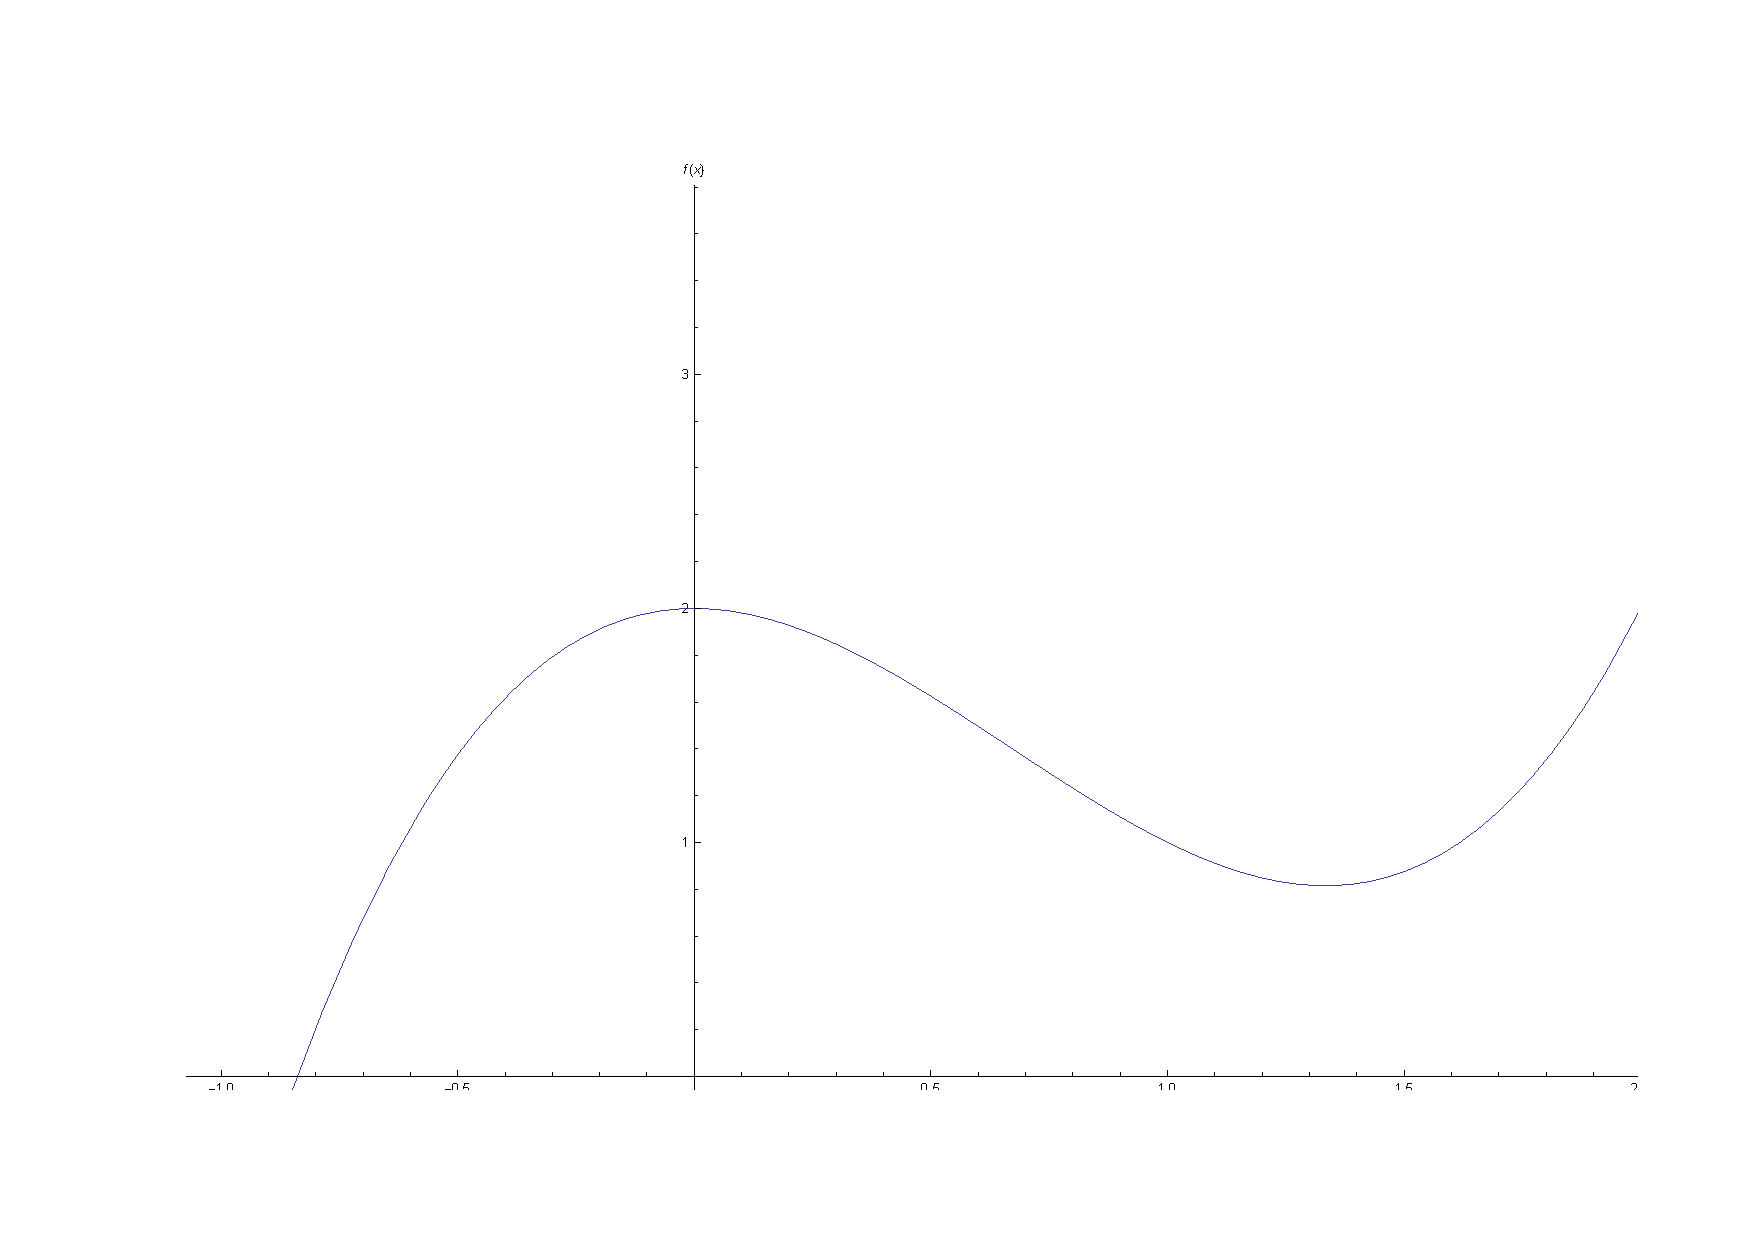
\includegraphics{img/grad1.pdf}
			}
		\end{subfigure}
		\begin{subfigure}{0.3\textwidth}
			\centering
			\resizebox{!}{0.7\linewidth}{
				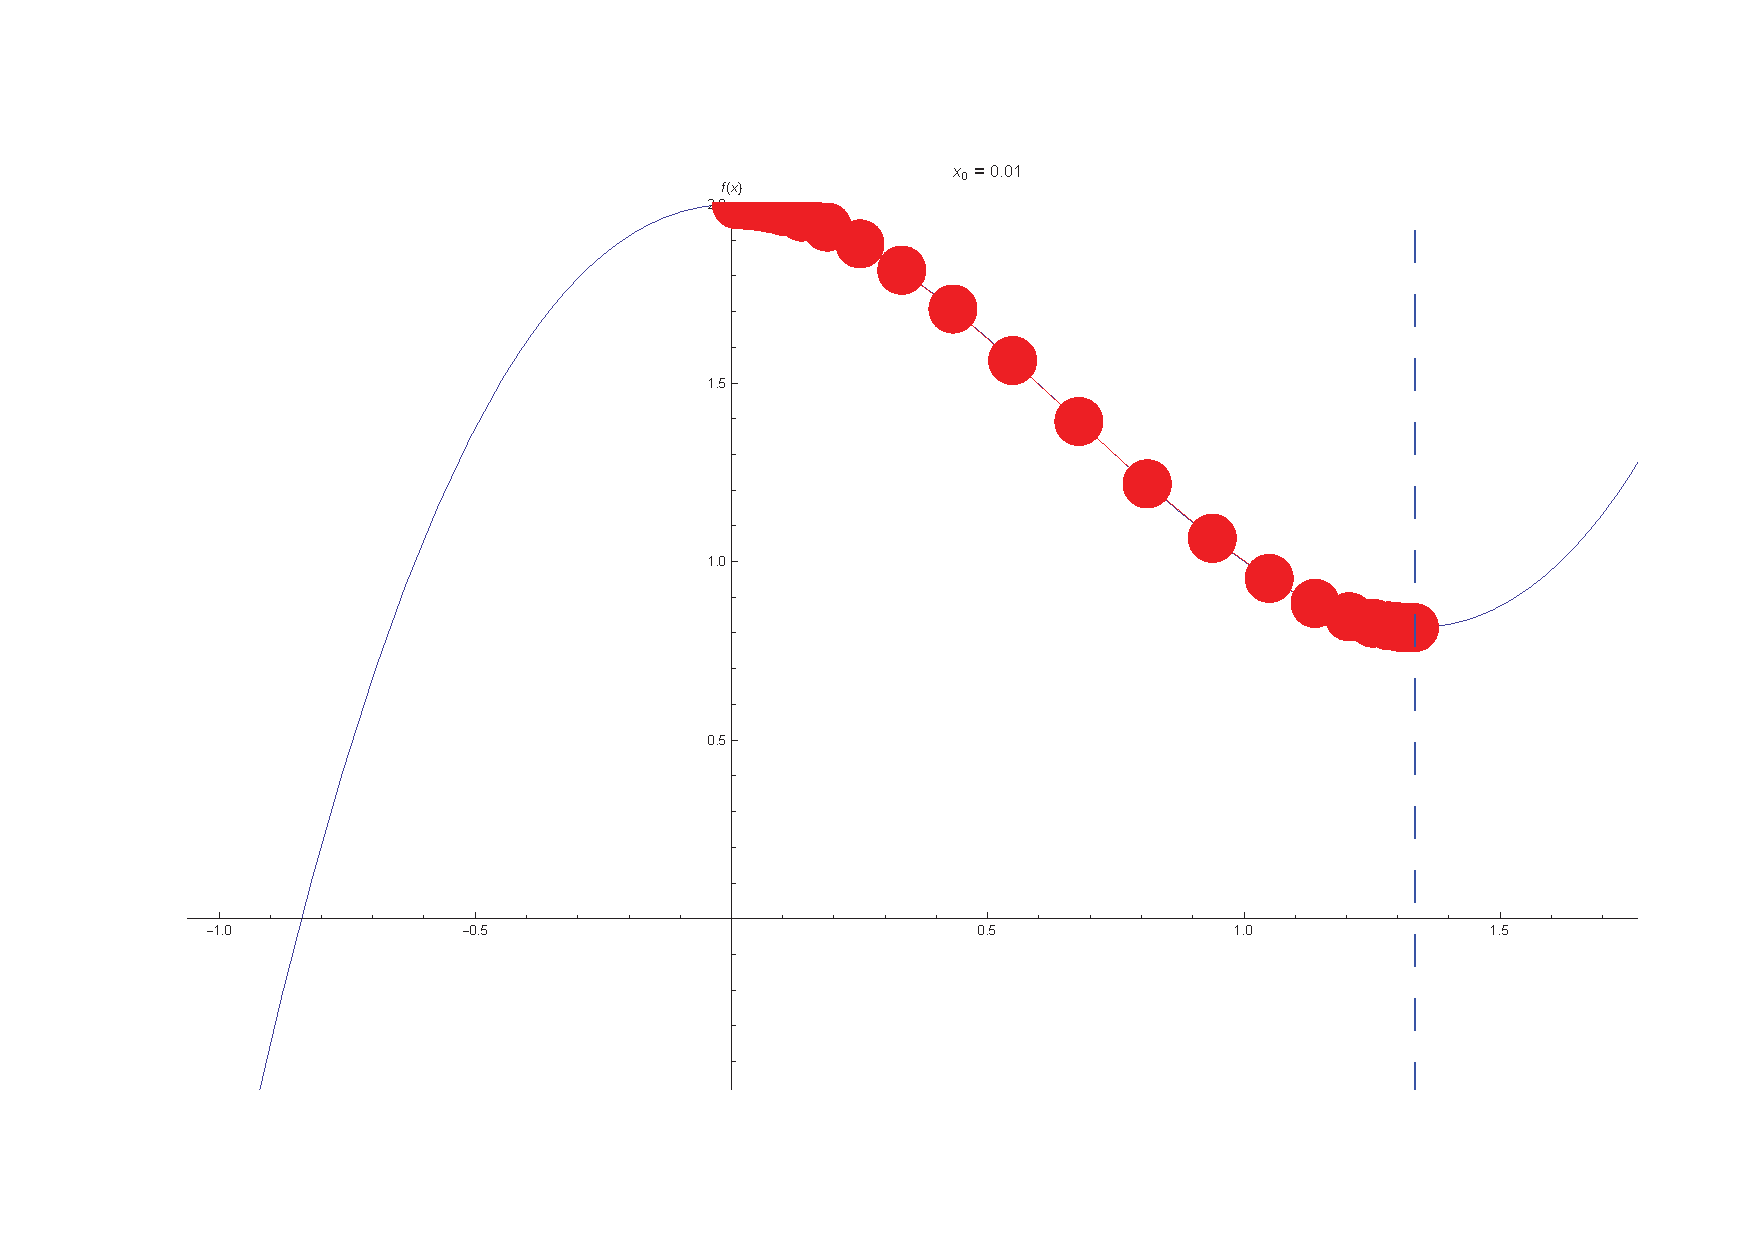
\includegraphics{img/grad2.pdf}
			}
		\end{subfigure}
		\begin{subfigure}{0.3\textwidth}
			\centering
			\resizebox{!}{0.7\linewidth}{
				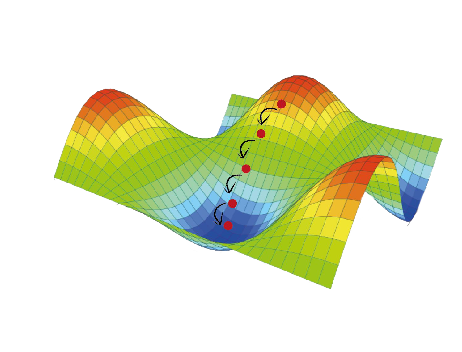
\includegraphics{img/3dgrad.png}
			}
		\end{subfigure}
		\caption{Função a minimizar (esquerda) e passos do método da descida mais rápida em 2-d e em 3-d (direita).}
	\end{figure}
	
    %% Notes:
    \note{-- Um gradiente positivo significa que reduzimos x. Um gradiente negativo significa que aumentamos x.
    
    -- Um algoritmo para encontrar o mínimo local mais próximo de uma função que pressupõe que o gradiente da função pode ser calculado.
    
    -- Depois de dar um passo, você olha novamente para a área ao redor para ver em qual direcção o aproxima de seu objectivo e, em seguida, dá um passo novamente nessa direcção. Continue fazendo isso até ficar feliz por ter chegado ao fundo do poço. O gradiente se refere à inclinação do solo. Você dá um passo na direcção em que a inclinação é mais acentuada para baixo

    -- É importante treinar a rede várias vezes e definir bem o passo. 
    
    }
    
\end{frame}
% #############################################################################

% #############################################################################
\begin{frame}{\textit{Backpropagation} \cont}
   
    O \textbf{gradiente do erro} para um determinado peso entre a última camada oculta e a camada de saída é dado por:
    \begin{equation}
        \frac{\partial E}{\partial w_{jk}} = -E_k \times O_k \times (1-O_k) \times o_j,
    \end{equation}
    onde $E_k = (y_k - \hat{y}_k)^2$, $O_k = \text{sigmóide}\left(\mathbf{w} \cdot \mathbf{i} \right)$ e $o_j$ é o valor de saída do neurónio anterior. 
    
    \pauseskip
    
    O \textbf{peso é, assim, actualizado} da seguinte forma:
    \begin{equation}
        w_{jk}' = w_{jk} - \alpha \times \frac{\partial E}{\partial w_{jk}},
    \end{equation}
    onde $\alpha$ é o \textit{learning rate}, tal como vimos anteriormente. 
    
    \pauseskip
    
    O \textit{learning rate} mede a deslocação (passo) ao longo da direcção $\frac{\partial E}{\partial w_{jk}}$.
    
    \pauseskip
    
    Esta técnica é considerada uma técnica de \textit{\alertbf{supervised learning}}.
    
    %% Notes:
    \note{-- É importante salientar que esta última expressão é uma expressão genéricas dos métodos de descida. 
    
    -- Diferentes escolhas para d, correspondem a distintos métodos iterativos, como por exemplo, método dos gradientes conjugados ou método de Newton, ou um dos mais conhecidos o de Levenberg--Marquardt.
    }
    
\end{frame}
% #############################################################################

% #############################################################################
\begin{frame}{\textit{Backpropagation} \cont}

    \begin{example}[Actualizar um peso de uma RNA:]
    
    \begin{figure}
        \centering
        \begin{tikzpicture}[shorten >=1pt,->,draw=black, node distance=\layersep]
    \tikzstyle{every pin edge}=[<-,shorten <=1pt]
    \tikzstyle{neuron}=[circle,minimum size=17pt, draw=black, inner sep=0pt]
    \tikzstyle{input neuron}=[neuron];
    \tikzstyle{output neuron}=[neuron];
    \tikzstyle{hidden neuron}=[neuron];
    \tikzstyle{annot} = [text width=5em, text centered]

    \path[yshift=0.5cm] node[hidden neuron, light-gray] (I-1) at (0,-1) {};
    \path[yshift=0.5cm] node[hidden neuron, light-gray] (I-2) at (0,-2) {};
    
    \path[yshift=0.5cm] node[hidden neuron] (H-1) at (\layersep,-1) {\scriptsize 0,4};
    \path[yshift=0.5cm] node[hidden neuron] (H-2) at (\layersep,-2) {\scriptsize 0,5};
    
    % Draw the hidden layer nodes
    \path[yshift=0.5cm] node[hidden neuron, pin={[pin edge={->}]right:$E_1 = 1,5$},] (O-1) at (2*\layersep,-1) {};
    \path[yshift=0.5cm] node[hidden neuron, light-gray] (O-2) at (2*\layersep,-2) {};
    
    % Connect every node in the hidden layer with the output layer
    \foreach \source in {1,...,2}
        \foreach \dest in {1,...,2}
            \path (I-\source) edge[light-gray] (H-\dest);

    \path (H-1) edge node[pos=.1,above]{\scriptsize 2} (O-1);
    \path (H-1) edge [light-gray] (O-2);
    
    \path (H-2) edge node[pos=.1,above]{\scriptsize 3} (O-1);
    \path (H-2) edge[light-gray] (O-2);

\end{tikzpicture}

    \end{figure}

    Vamos considerar $E_1 = 1,5$ e actualizar o peso $w_{11}$.
    
    \pauseskip
    
    O somatório vem:
    \begin{equation}
        \sum_{j=1}^2 w_{j1} i_1 = w_{11} \times i_1 + w_{21} \times i_1 = (2 \times 0,4) + (3 \times 0,5) = 2,3. 
    \end{equation}
    
    \pauseskip
    
    Aplicando a função sigmóide, $\text{sigmóide}(2,3) = 0,909 = O_1$.
    
    \end{example}

\end{frame}
% #############################################################################

% #############################################################################
\begin{frame}{\textit{Backpropagation} \cont}

    \begin{example}[Actualizar um peso de uma RNA---continuação:]
    
    \begin{figure}
        \centering
        \begin{tikzpicture}[shorten >=1pt,->,draw=black, node distance=\layersep]
    \tikzstyle{every pin edge}=[<-,shorten <=1pt]
    \tikzstyle{neuron}=[circle,minimum size=17pt, draw=black, inner sep=0pt]
    \tikzstyle{input neuron}=[neuron];
    \tikzstyle{output neuron}=[neuron];
    \tikzstyle{hidden neuron}=[neuron];
    \tikzstyle{annot} = [text width=5em, text centered]

    \path[yshift=0.5cm] node[hidden neuron, light-gray] (I-1) at (0,-1) {};
    \path[yshift=0.5cm] node[hidden neuron, light-gray] (I-2) at (0,-2) {};
    
    \path[yshift=0.5cm] node[hidden neuron] (H-1) at (\layersep,-1) {\scriptsize 0,4};
    \path[yshift=0.5cm] node[hidden neuron] (H-2) at (\layersep,-2) {\scriptsize 0,5};
    
    % Draw the hidden layer nodes
    \path[yshift=0.5cm] node[hidden neuron, pin={[pin edge={->}]right:$E_1 = 1,5$},] (O-1) at (2*\layersep,-1) {};
    \path[yshift=0.5cm] node[hidden neuron, light-gray] (O-2) at (2*\layersep,-2) {};
    
    % Connect every node in the hidden layer with the output layer
    \foreach \source in {1,...,2}
        \foreach \dest in {1,...,2}
            \path (I-\source) edge[light-gray] (H-\dest);

    \path (H-1) edge node[pos=.1,above]{\scriptsize 2} (O-1);
    \path (H-1) edge [light-gray] (O-2);
    
    \path (H-2) edge node[pos=.1,above]{\scriptsize 3} (O-1);
    \path (H-2) edge[light-gray] (O-2);

\end{tikzpicture}

    \end{figure}

    Desta forma,
    \begin{equation}
        \begin{split}
             \frac{\partial E}{\partial w_{11}} &= -E_1 \times O_1 \times (1-O_1) \times {o_1}_{\; \text{(anterior)}} \\
            &= -1,5 \times 0,909 \times (1 - 0,909)\times0,4 = -0,049.
        \end{split}
    \end{equation}
    
    \pauseskip
    
    Juntando tudo na equação final, e considerando um \textit{learning rate} de 0,1, temos
    \begin{equation}
        w_{11}' = w_{11} - \alpha \times \frac{\partial E}{\partial w_{11}} =  2 - 0,1 \times (-0,049) = 2,005.
    \end{equation}
        
    \end{example}

\end{frame}
% #############################################################################

% #############################################################################
\begin{frame}{\textit{Backpropagation} \cont}

Para os restantes pesos, a expressão é semelhante, e é dada por 
\begin{equation}
    \frac{\partial E}{\partial w_{jk}} = -e_k \times O_k \times (1-O_k) \times o_j,
\end{equation}
onde $e_k$ é o erro que vem da retropropagação. 

\pauseskip

Contudo, no caso genérico, têm-se
\begin{equation}
	\frac{\partial E}{\partial w_{jk}} = -e_k \times \frac{\partial}{\partial w_{jk}}\phi\left(\sum_j  w_{jk} \cdot o_{j}\right)\times o_j,
\end{equation}
onde $\phi$ é, tal como vimos, uma qualquer função de activação diferenciável.  

\end{frame}
% #############################################################################

% #############################################################################
\begin{frame}{\textit{Backpropagation} \cont}
    
    Na prática, o método da descida mais rápida \textbf{não é utilizado directamente para o treino de uma RNA}.
    
    \pauseskip
    
    Como alternativa, podemos usar o método do \alertbf{gradiente descendente estocástico} (SGD). 
    
    \pauseskip
    
    O SGD utiliza uma \textbf{aproximação do gradiente} da função calculado a partir de um \textbf{subconjunto de dados (\textit{batch}) seleccionado aleatoriamente} (\textit{mini-batch}).
    
    \pauseskip
    
    Uma \textbf{passagem por todos os \textit{mini-batches}} de um conjunto de dados designa-se por \alertbf{\textit{época}}.
    
\end{frame}
% #############################################################################

% #############################################################################
\begin{frame}{\textit{Backpropagation} \cont}
    
    \begin{figure}
        \centering
        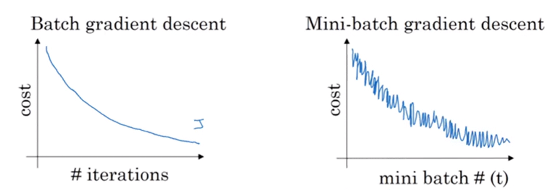
\includegraphics[width=0.7\textwidth]{img/grad_descent.png}
        \caption{Diferença entre o método da descida e o gradiente descendente estocástico.}
    \end{figure}
    
    \pauseskip
    
    É preciso ter em atenção que:
    \begin{itemize}
        \item \textit{mini-batches} com um \textbf{número pequeno de registos} faz com que o algoritmo precise de \textbf{mais iterações para convergir}.
        \medskip
        \item \textit{mini-batches} com um \textbf{número grande de registos} faz com que o cálculo do gradiente seja \textbf{mais exacto}, contudo \textbf{mais lento}.
    \end{itemize}
    
\end{frame}
% #############################################################################

% #############################################################################
\begin{frame}{\textit{Backpropagation} \cont}
    
    É, ainda, possível \textbf{obter os pesos quase-óptimos} de uma RNA \textbf{sem recorrer ao cálculo de derivadas}.
    
    \pauseskip
    
    Estes métodos constituem \textbf{técnicas tradicionais de optimização}, tais como:
    \begin{itemize}
        \item Enxame de partículas;
        \medskip
        \item Algoritmos genéticos;
        \medskip
        \item Arrefecimento simulado.
    \end{itemize}

    \pauseskip
    
    A vantagem destes algoritmos é que podemos \textbf{optimizar a arquitectura de uma RNA e os seus pesos}.
    
    %% Notes:
    \note{Os algoritmos sem derivada podem demorar mais tempo a convergir.}
    
\end{frame}
% #############################################################################

% #############################################################################
\begin{frame}{\textit{Forward} e \textit{Backpropagation}}
    \textbf{Vamos rever:}
    
    \medskip
    
    \begin{enumerate}
        \item  Os neurónios de entrada recebem os valores de entrada e os transmitem para a camada oculta seguinte.
        \pauseskip
        \item Com base numa função matemática, cada neurónio oculto produz um valor e passa esse valor para a próxima camada oculta (se existir) ou para a camada de saída.
        \pauseskip
        \item A camada de saída recebe as saídas da última camada oculta e calcula o valor previsto pelo modelo.
        \pauseskip
        \item Este valor previsto é, então, comparado com o valor esperado, e o erro é usado para actualizar os pesos das conexões sinápticas, com base num algoritmo de optimização.
    \end{enumerate}
    
\end{frame}
% #############################################################################

% #############################################################################
\section{Classificação vs. Regressão}
% #############################################################################

% #############################################################################
\begin{frame}{Classificação vs. Regressão}

Classificação e regressão \textbf{são problemas semelhantes}.

\medskip

Em termos gerais, a classificação tenta \textbf{rotular} uma combinação de características. Por outro lado, a regressão tenta estimar uma \textbf{quantidade}.

\pauseskip

Exemplos:
\begin{itemize}
    \item \textbf{Regressão:} previsão do preço de uma casa, da altura de uma pessoa, do preço de acções\ldots
    \item \textbf{Classificação:} detecção de correio electrónico não solicitado, reconhecimento de algarismos, reconhecimento de espécies\ldots
\end{itemize}

\end{frame}
% #############################################################################  

% #############################################################################
\begin{frame}{Classificação vs. Regressão \cont}

Apesar de problemas de classificação lidarem com varáveis discretas, \textbf{a saída da rede neuronal é contínua}.

\pauseskip

Se for usada a função de activação correcta, esta saída é vista como uma \textbf{probabilidade de uma dada combinação de características pertencer a uma dada classe}.

\begin{figure}
    \centering
    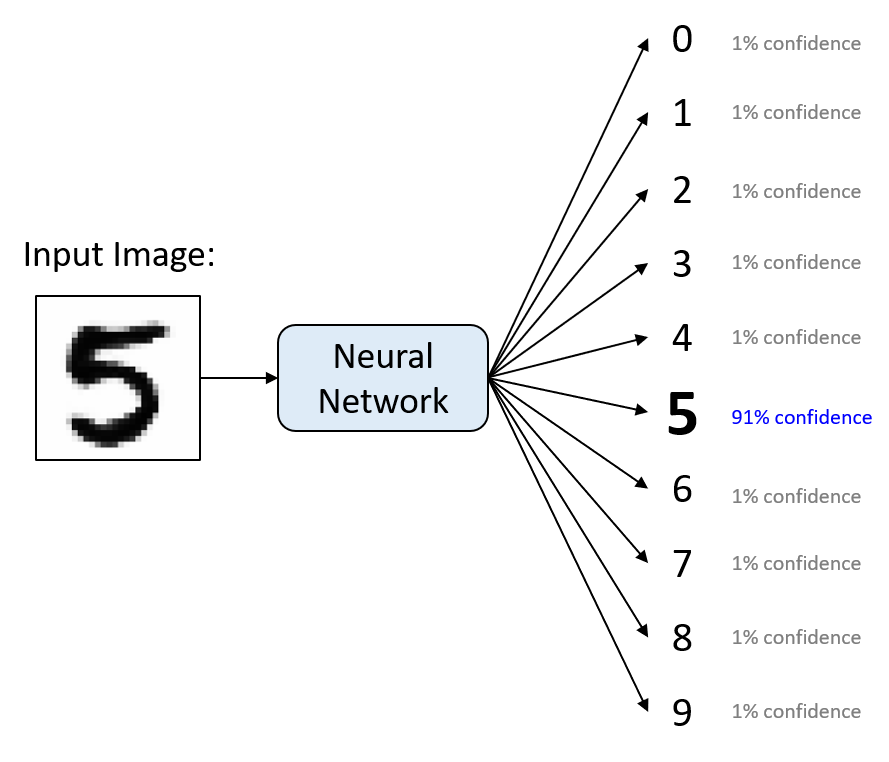
\includegraphics[width=4.5cm]{img/classification.png}
    \caption{Exemplo de um problema de classificação.}
\end{figure}

%% Notes:
\note{A classe que depois irá ser associada à combinação corresponde à classe como maior probabilidade.

O número de saídas da rede neuronal corresponde ao número de classes.
}

\end{frame}
% #############################################################################

% #############################################################################
\begin{frame}{Classificação vs. Regressão \cont}

\alertbf{Como podemos estimar a capacidade do nosso modelo de classificação?}

\bigskip

\begin{columns}
    \begin{column}{0.48\textwidth}
        \resizebox{!}{0.4\textwidth}{
    \begin{tabular}{c >{\bfseries}r @{\hspace{0.7em}}c @{\hspace{0.4em}}c @{\hspace{0.7em}}l}
      \multirow{10}{*}{\parbox{1.1cm}{\bfseries\raggedleft Classe\\ Real}} & 
        & \multicolumn{2}{c}{\bfseries Classe Prevista} & \\
      & & \bfseries p & \bfseries n & \bfseries Total \\
      & p$'$ & \MyBox{Verdadeiro}{Positivo} & \MyBox{Falso}{Negativo} & P$'$ \\[2.4em]
      & n$'$ & \MyBox{Falso}{Positivo} & \MyBox{Verdadeiro}{Negativo} & N$'$ \\
      & Total & P & N &
    \end{tabular}
    }
    \end{column}
    \begin{column}{0.48\textwidth}
    
    Uma das medidas mais comuns é a \textit{accuracy}, e é dada por:
        \begin{equation}
            \text{ACC} = \dfrac{VP + VN}{P + N}.
        \end{equation}
    \end{column}
\end{columns}

\end{frame}
% #############################################################################

% #############################################################################
\begin{frame}{Classificação vs. Regressão \cont}

\alertbf{Como podemos estimar a capacidade do nosso modelo de regressão?}

\bigskip

\textbf{Existem várias métricas}, mas as mais comuns são o \textbf{erro quadrático médio (MSE)} e a \textbf{raiz do erro quadrático médio (RMSE)}.

\pauseskip

Estas métricas são definas da seguinte forma:
\begin{equation}
\begin{split}
    \text{MSE} &= \dfrac{1}{n} \sum_{k=1}^{n} (y_k - \hat{y}_k)^2 \quad \text{e} \\
    \text{RMSE} &= \sqrt{\text{MSE}}  = \sqrt{\dfrac{1}{n} \sum_{k=1}^{n} (y_k - \hat{y}_k)^2},
\end{split}
\end{equation}
onde $n$ é o número de amostras.

\end{frame}
% #############################################################################

% #############################################################################
\begin{frame}{Classificação vs. Regressão \cont}

Um vez que os modelos de \textbf{classificação} têm como valor de saída uma probabilidade, a \textbf{função de activação da camada de saída tem de estar no intervalo} $[0, 1]$.

\pauseskip

Para esse caso, um exemplo de função de activação a usar é a \textbf{função sigmóide}. 

\pauseskip

Para o caso da \textbf{regressão}, a última camada tem de possuir a \textbf{função de activação de identidade}, de modo a não restringir a \textbf{saída da rede ao domínio da função de activação}. 

\pauseskip

Na maioria dos casos, para as \textbf{camadas ocultas}, \textbf{qualquer função de activação} poderá ser usada. 

\end{frame}
% #############################################################################

% #############################################################################
\section{\textit{Overfitting} vs. \textit{Underfitting}}
% #############################################################################

% #############################################################################
\begin{frame}{\textit{Overfitting} vs. \textit{Underfitting}}
    
    O \textbf{objectivo} de qualquer modelo de \textit{machine learning} é \textbf{ter uma boa capacidade de generalização}.
    
    \pauseskip
    
    Assim, surge o conceito de \alertbf{\textit{overfitting}} e de \alertbf{\textit{underfitting}}:
    \begin{itemize}
        \item \textbf{\textit{Overfitting}}---quando o modelo se ajusta muito bem ao conjunto de dados de treino.
        \medskip
        \item \textbf{\textit{Underfitting}}---quando o modelo não se ajusta ao conjunto de dados de treino, nem de teste (modelo inadequado).
    \end{itemize}
    
    \medskip
    
    \begin{figure}
		\centering
		\begin{subfigure}{0.3\textwidth}
			\centering
			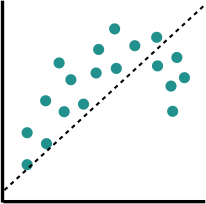
\includegraphics[width=0.7\linewidth]{img/underfit.png}
			\caption{\textit{Underfitting}.}
		\end{subfigure}
	    \begin{subfigure}{0.3\textwidth}
			\centering
			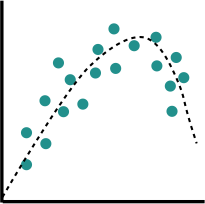
\includegraphics[width=0.7\linewidth]{img/optimal.png}
			\caption{Ponto óptimo.}
		\end{subfigure}
		\begin{subfigure}{0.3\textwidth}
			\centering
			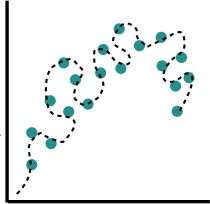
\includegraphics[width=0.7\linewidth]{img/overfit.png}
			\caption{\textit{Overfitting}.}
		\end{subfigure}
	\end{figure}
    
    %% Notes
    \note{-- Explicar os diferentes conjuntos: treino e teste.
    
    -- Underfitting - A solução é seguir em frente e tentar algoritmos alternativos de aprendizado de máquina. 
    
    }
    
\end{frame}
% #############################################################################

% #############################################################################
\begin{frame}{\textit{Overfitting} vs. \textit{Underfitting} \cont}
    
    O \textbf{ponto óptimo} é ter um \textbf{equilíbrio entre \textit{overfitting} e \textit{underfitting}}.
    
    \begin{figure}
        \centering
        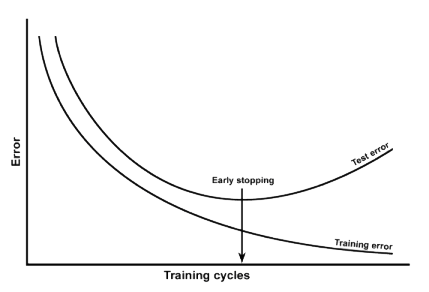
\includegraphics[width=0.45\linewidth]{img/estop.png}
        \caption{Ponto óptimo para paragem (antecipada) do treino.}
    \end{figure}

    \pause

    \begin{exampleblock}{Paragem (antecipada) do treino:}
        É uma técnica que consiste em interromper o treino antes que o modelo se torne excessivamente especializado nos dados de treino (\textit{overfitting}), garantindo que ainda mantenha a capacidade de generalizar bem para dados novos e não vistos (evitando \textit{underfitting}).
    \end{exampleblock}
    
\end{frame}
% #############################################################################

% #############################################################################
\section{Validação de Modelo}
% #############################################################################

% #############################################################################
\begin{frame}{Validação de Modelo}

    Para validar um modelo, usamos comummente um conjunto de \alertbf{dados de treino} e um \alertbf{conjunto de dados de teste}.

    \medskip
    
    O conjunto de dados de teste \textbf{não é usado para treinar o modelo}.

    \pauseskip
    
    A avaliação do modelo usando o \textbf{conjunto de dados de teste é o mais interessante de reportar}, uma vez que o modelo está a \enquote{ver} pela primeira vez esse conjunto de dados.

    \medskip
    
    Dessa forma, estamos a \alertbf{avaliar a capacidade de generalização do modelo}. 
    
    \textbf{Exemplos de métodos:} $n$-\textit{Fold Cross-Validation} e \textit{Leave-One-Out Cross-Validation}. 

\end{frame}
% #############################################################################

% #############################################################################
\section{Outros Tipos de Redes}
% #############################################################################

% #############################################################################
\begin{frame}{LSTMs}

A \textbf{estrutura de uma rede \textit{Long Short Term Memory}~(LSTM)} é a seguinte\footnote{\tiny{Imagem adaptada de: https://colah.github.io/posts/2015-08-Understanding-LSTMs}}:

\begin{figure}
    \centering
    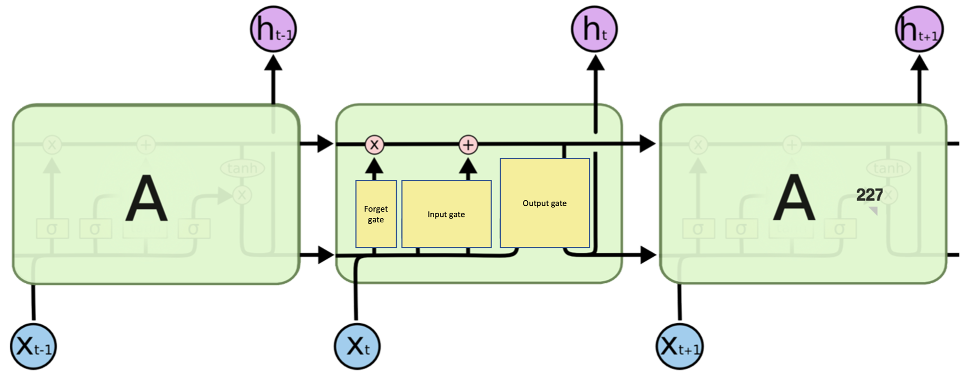
\includegraphics[width=0.8\textwidth]{img/LSTM.png}
\end{figure}

\pause

São modelos úteis quando existe uma \textbf{sequência ordenada nos dados}, pois conseguem guardar \textbf{contexto}, \textit{i.e.}, quando os valores do passado poderão ajudar a predizer os valores do futuro.

%% Notes
\note{-- As LSTMs devem ser usadas quando existem uma sequência nos dados. Por exemplo, séries temporais. Onde os valores do passado, poderão ajudar a predizer os valores do futuro.
-- Com uma LSTM é possível dar à rede um contexto, e quanto maior for o contexto, mais facilidade a rede terá de predizer a próxima sequência.}

\end{frame}
% #############################################################################

% #############################################################################
\begin{frame}{LSTMs \cont}

\begin{figure}
    \centering
    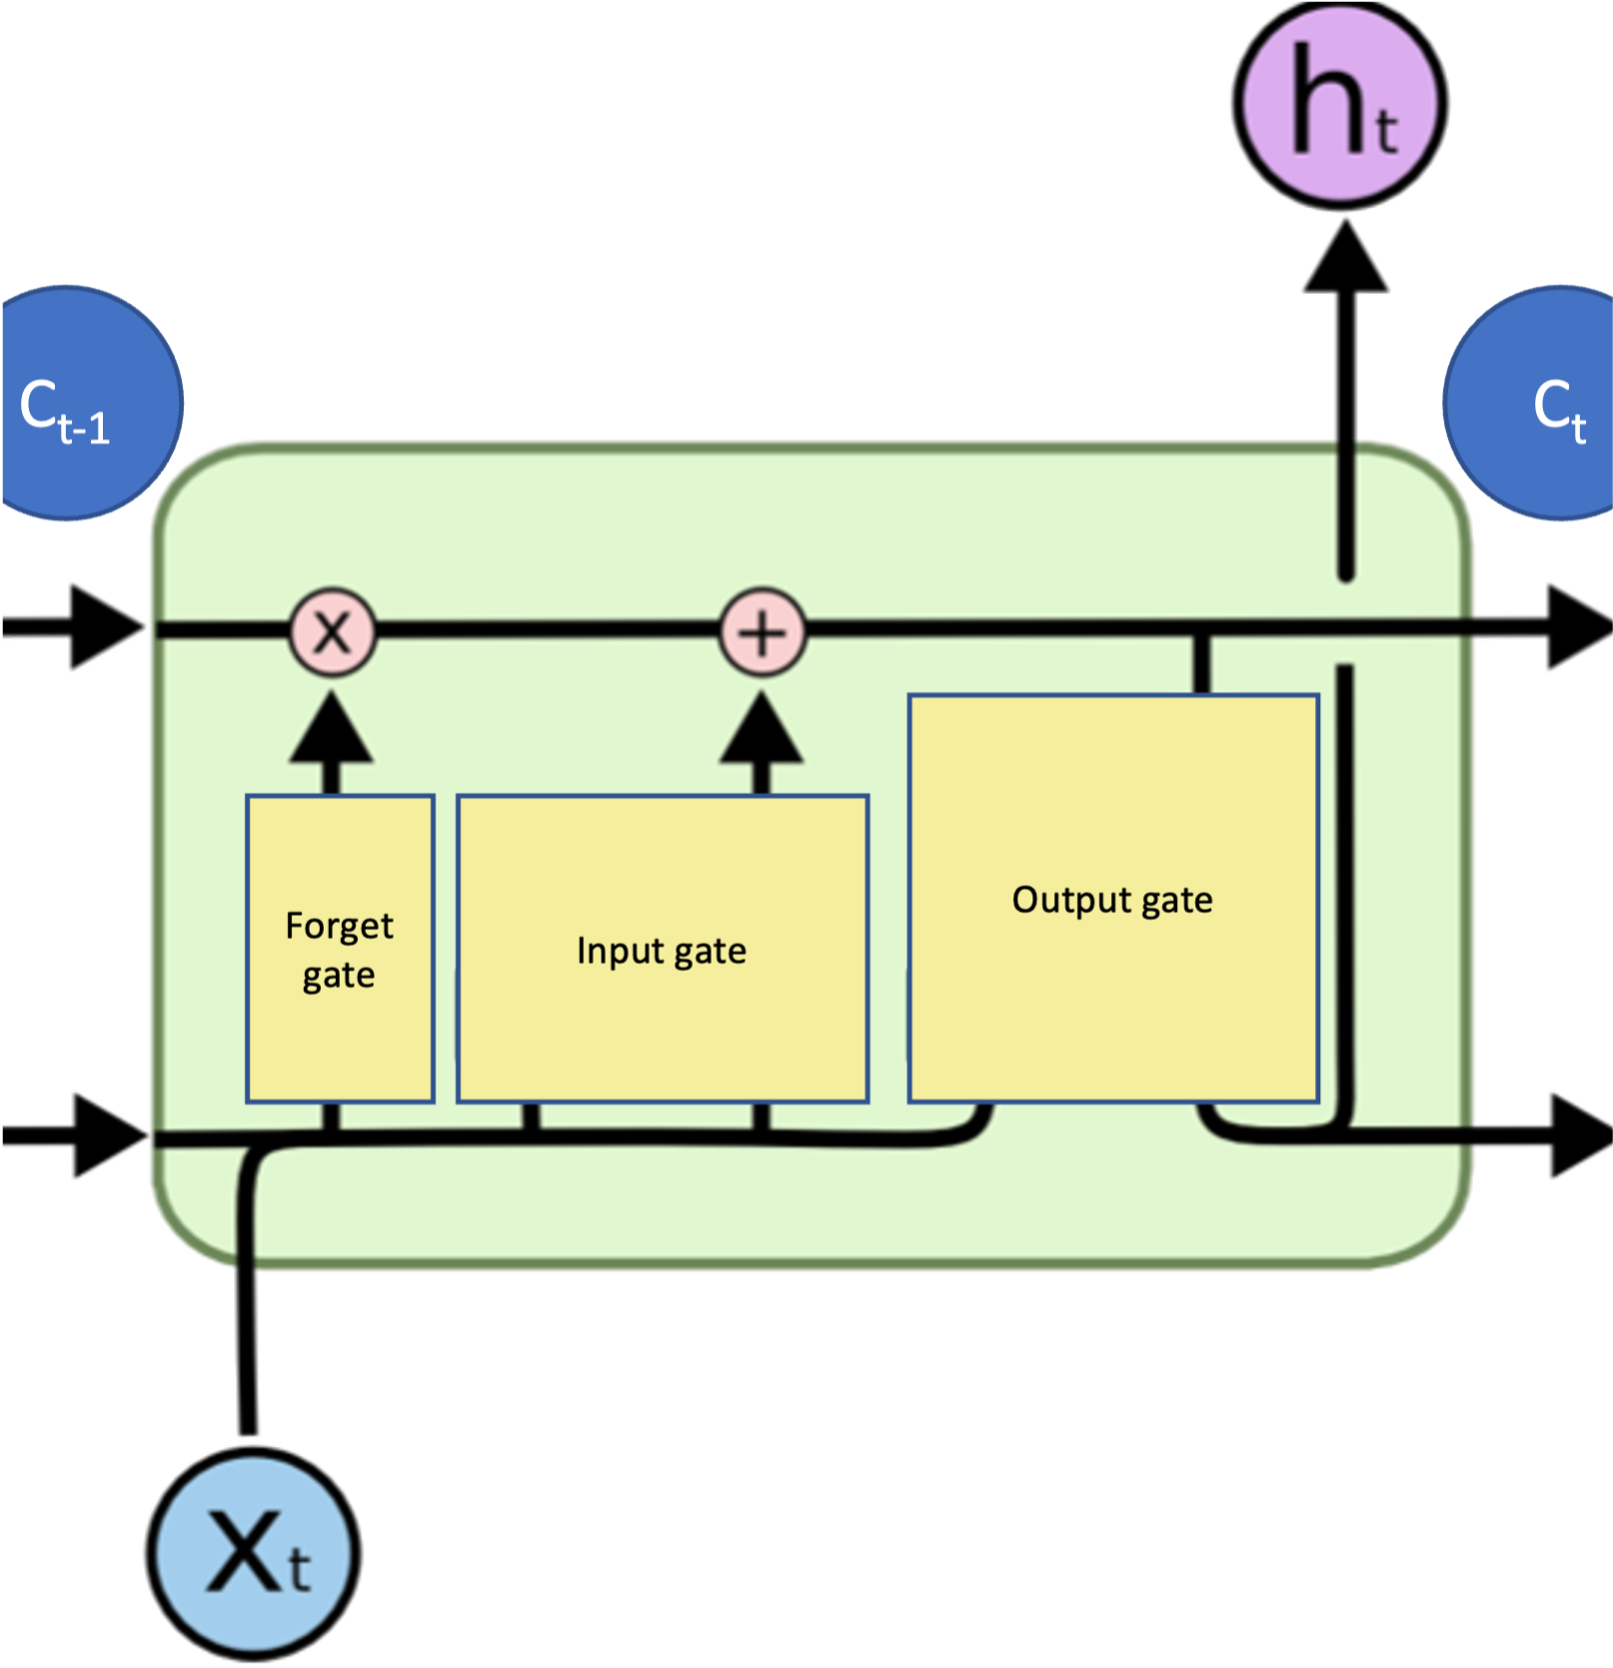
\includegraphics[width=0.35\textwidth]{img/LSTMSingle.png}
\end{figure}

Cada célula de uma \textbf{LSTM possui três operações/portas} (\textit{gates}):
\begin{itemize}
    \item \textit{\textbf{forget}}---que informação esquecer?
    \pause
    \item \textit{\textbf{input}}---o que adicionar ao que já sei?
    \pause
    \item \textit{\textbf{output}}---que informação passar?
\end{itemize}

\pauseskip

\alertbf{Este tipo de redes consegue aprender dependências douradoras, bem como esporádicas.}

%% Notes:
\note{Forget---responsável por decidir que \textbf{informação esquecer ou manter} do estado anterior. No fundo, guarda keywords. E esquece as palavras de ligação.
Input---responsável por \textbf{adicionar mais informação} ao estado actual.
Output---responsável por \textbf{calcular estado oculto}. No fundo, pode passar características do dos sujeitos, etc.
-- Por exemplo, fraudes com o cartão de crédito. Se por exemplo, eu nunca fiz um levantamento de nunca mais do que 500 euros, se fizer um, é bem provável que seja fraudulento.}

\end{frame}
% #############################################################################

% #############################################################################
\begin{frame}{CNNs}

A \textbf{estrutura de uma rede \textit{Convolutional Neural Network}~(CNN)} é a seguinte\footnote{\tiny{Imagem retirada de: https://developer.qualcomm.com/software/qualcomm-neural-processing-sdk/learning-resources/cnn-architectures/deep-learning-convolutional-neural-networks-computer-vision}}:

\begin{figure}
    \centering
    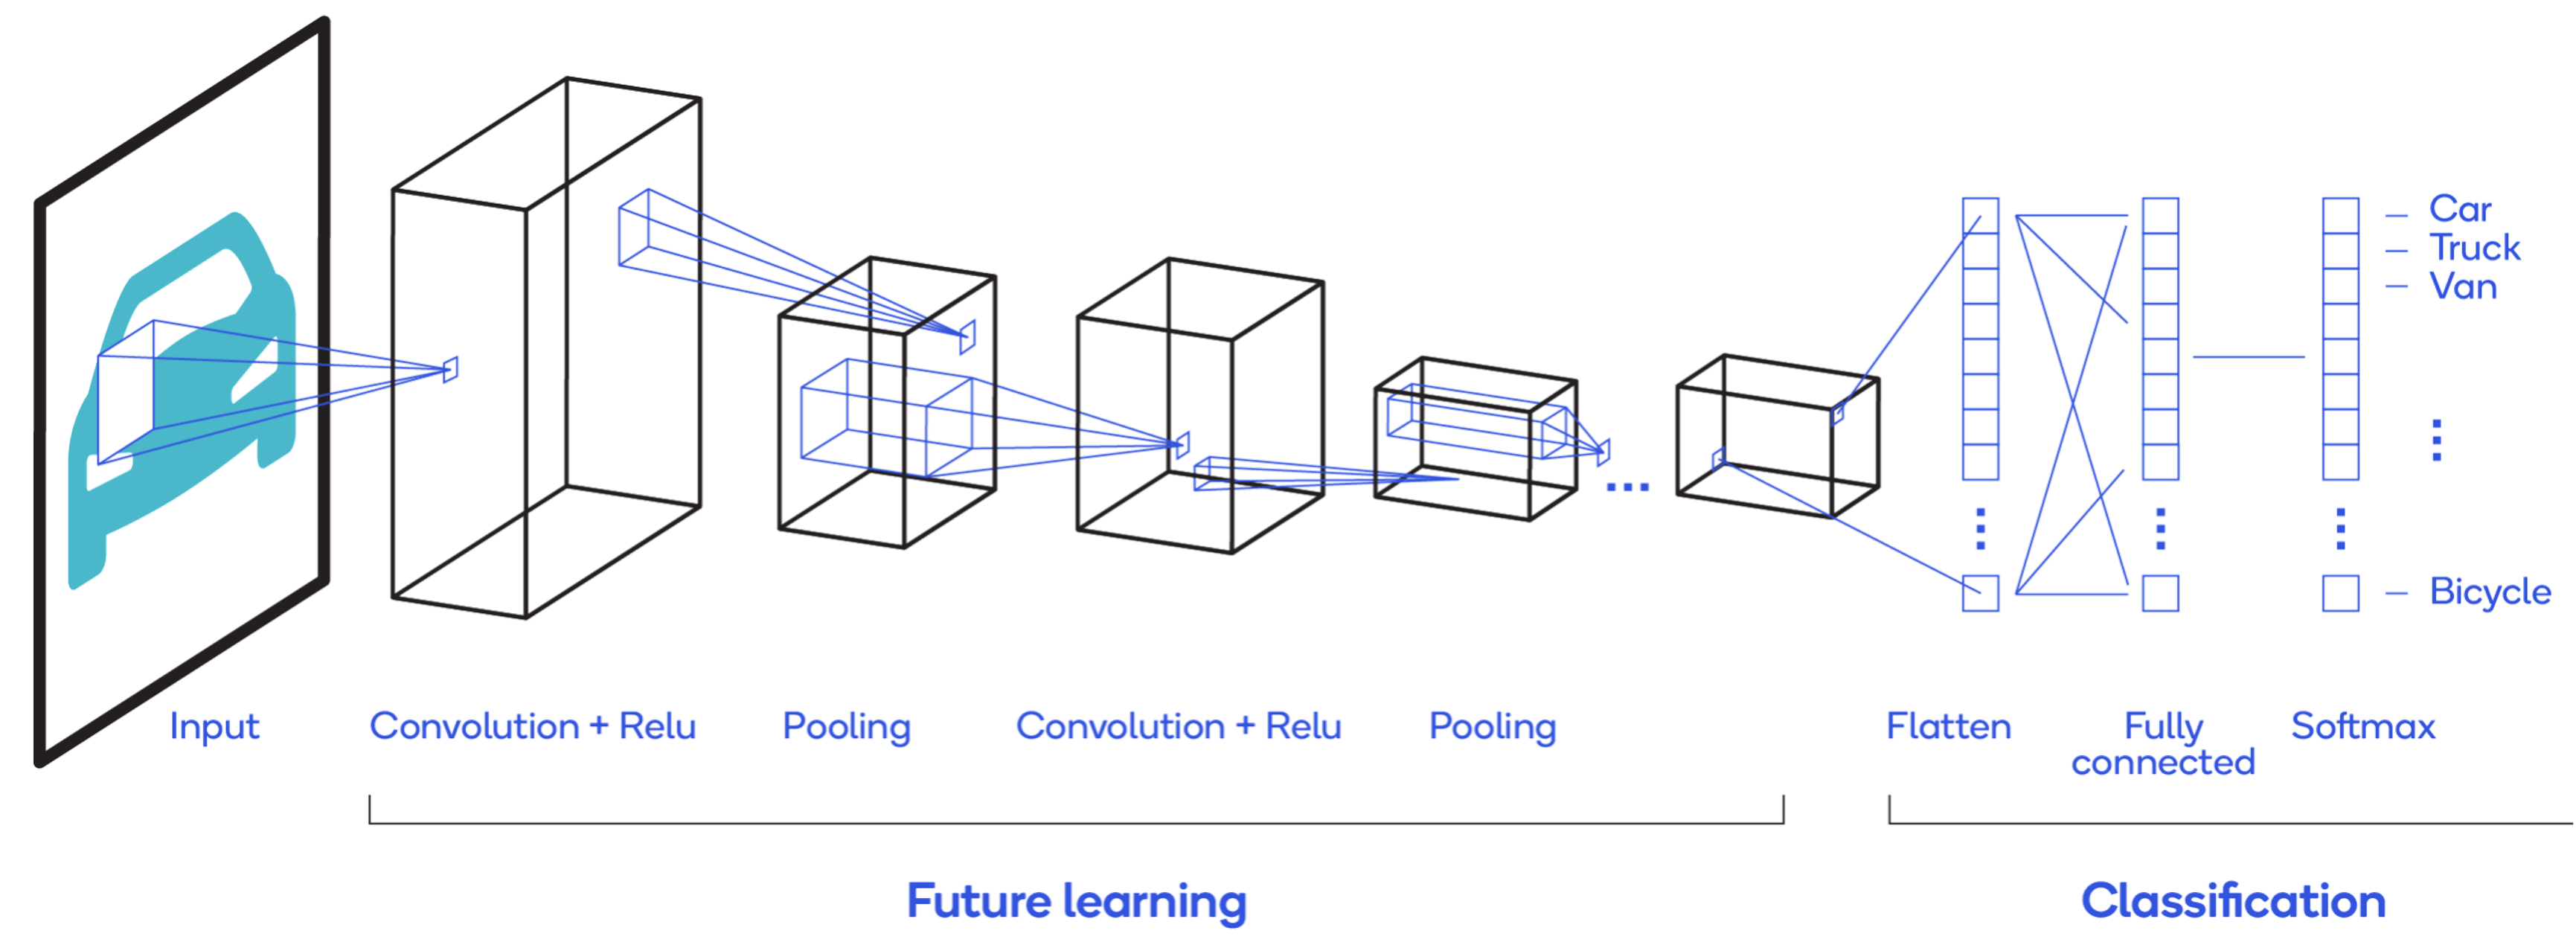
\includegraphics[width=0.75\textwidth]{img/CNN.png}
\end{figure}

São modelos usados para aplicações de \textit{computer vision}, e \textbf{têm o objectivo de imitar}, pela interpretação de informações presentes em imagens, vídeos ou áudio, \textbf{a visão humana}.

\end{frame}
% #############################################################################

% #############################################################################
\begin{frame}{CNNs \cont}

    \begin{columns}[T,onlytextwidth]
    \column{0.45\textwidth}

    \begin{figure}
        \centering
        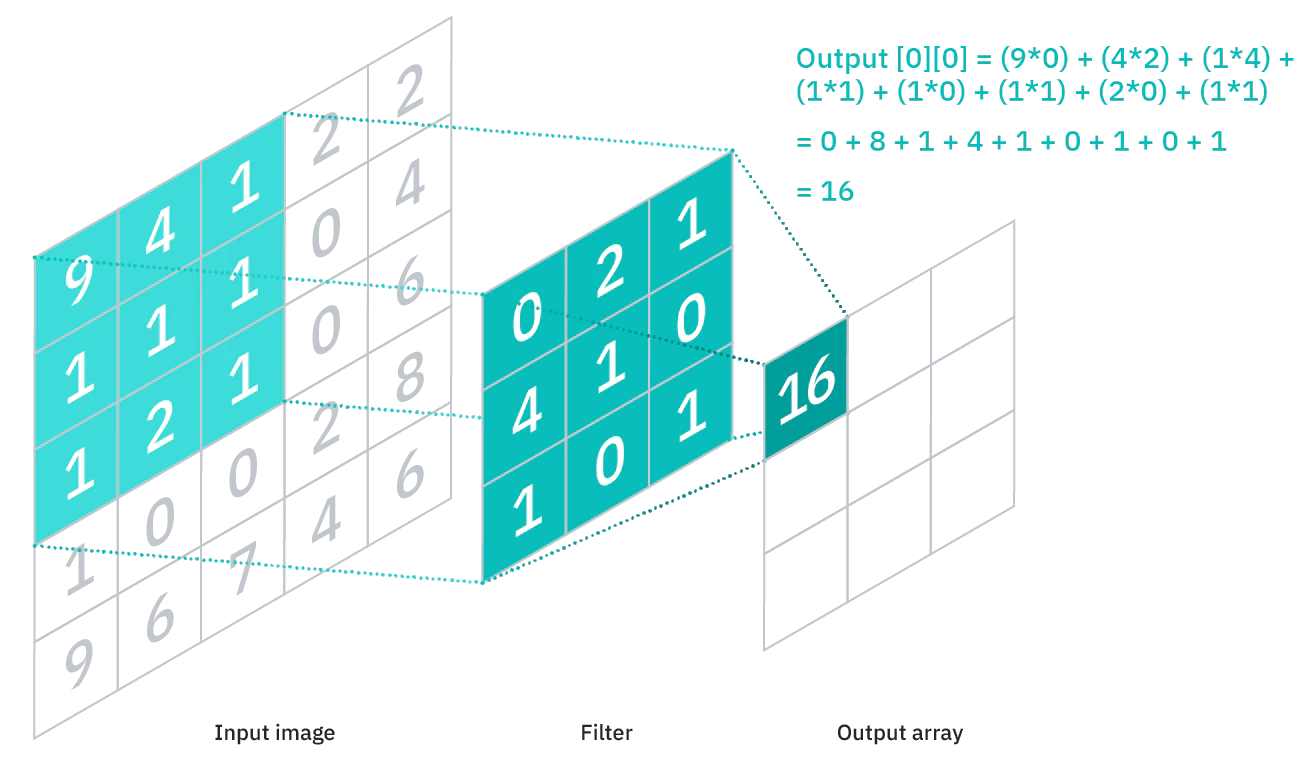
\includegraphics[width=\textwidth]{img/convolution.png}
    \end{figure}

    \column{0.5\textwidth}

    \begin{figure}
        \centering
        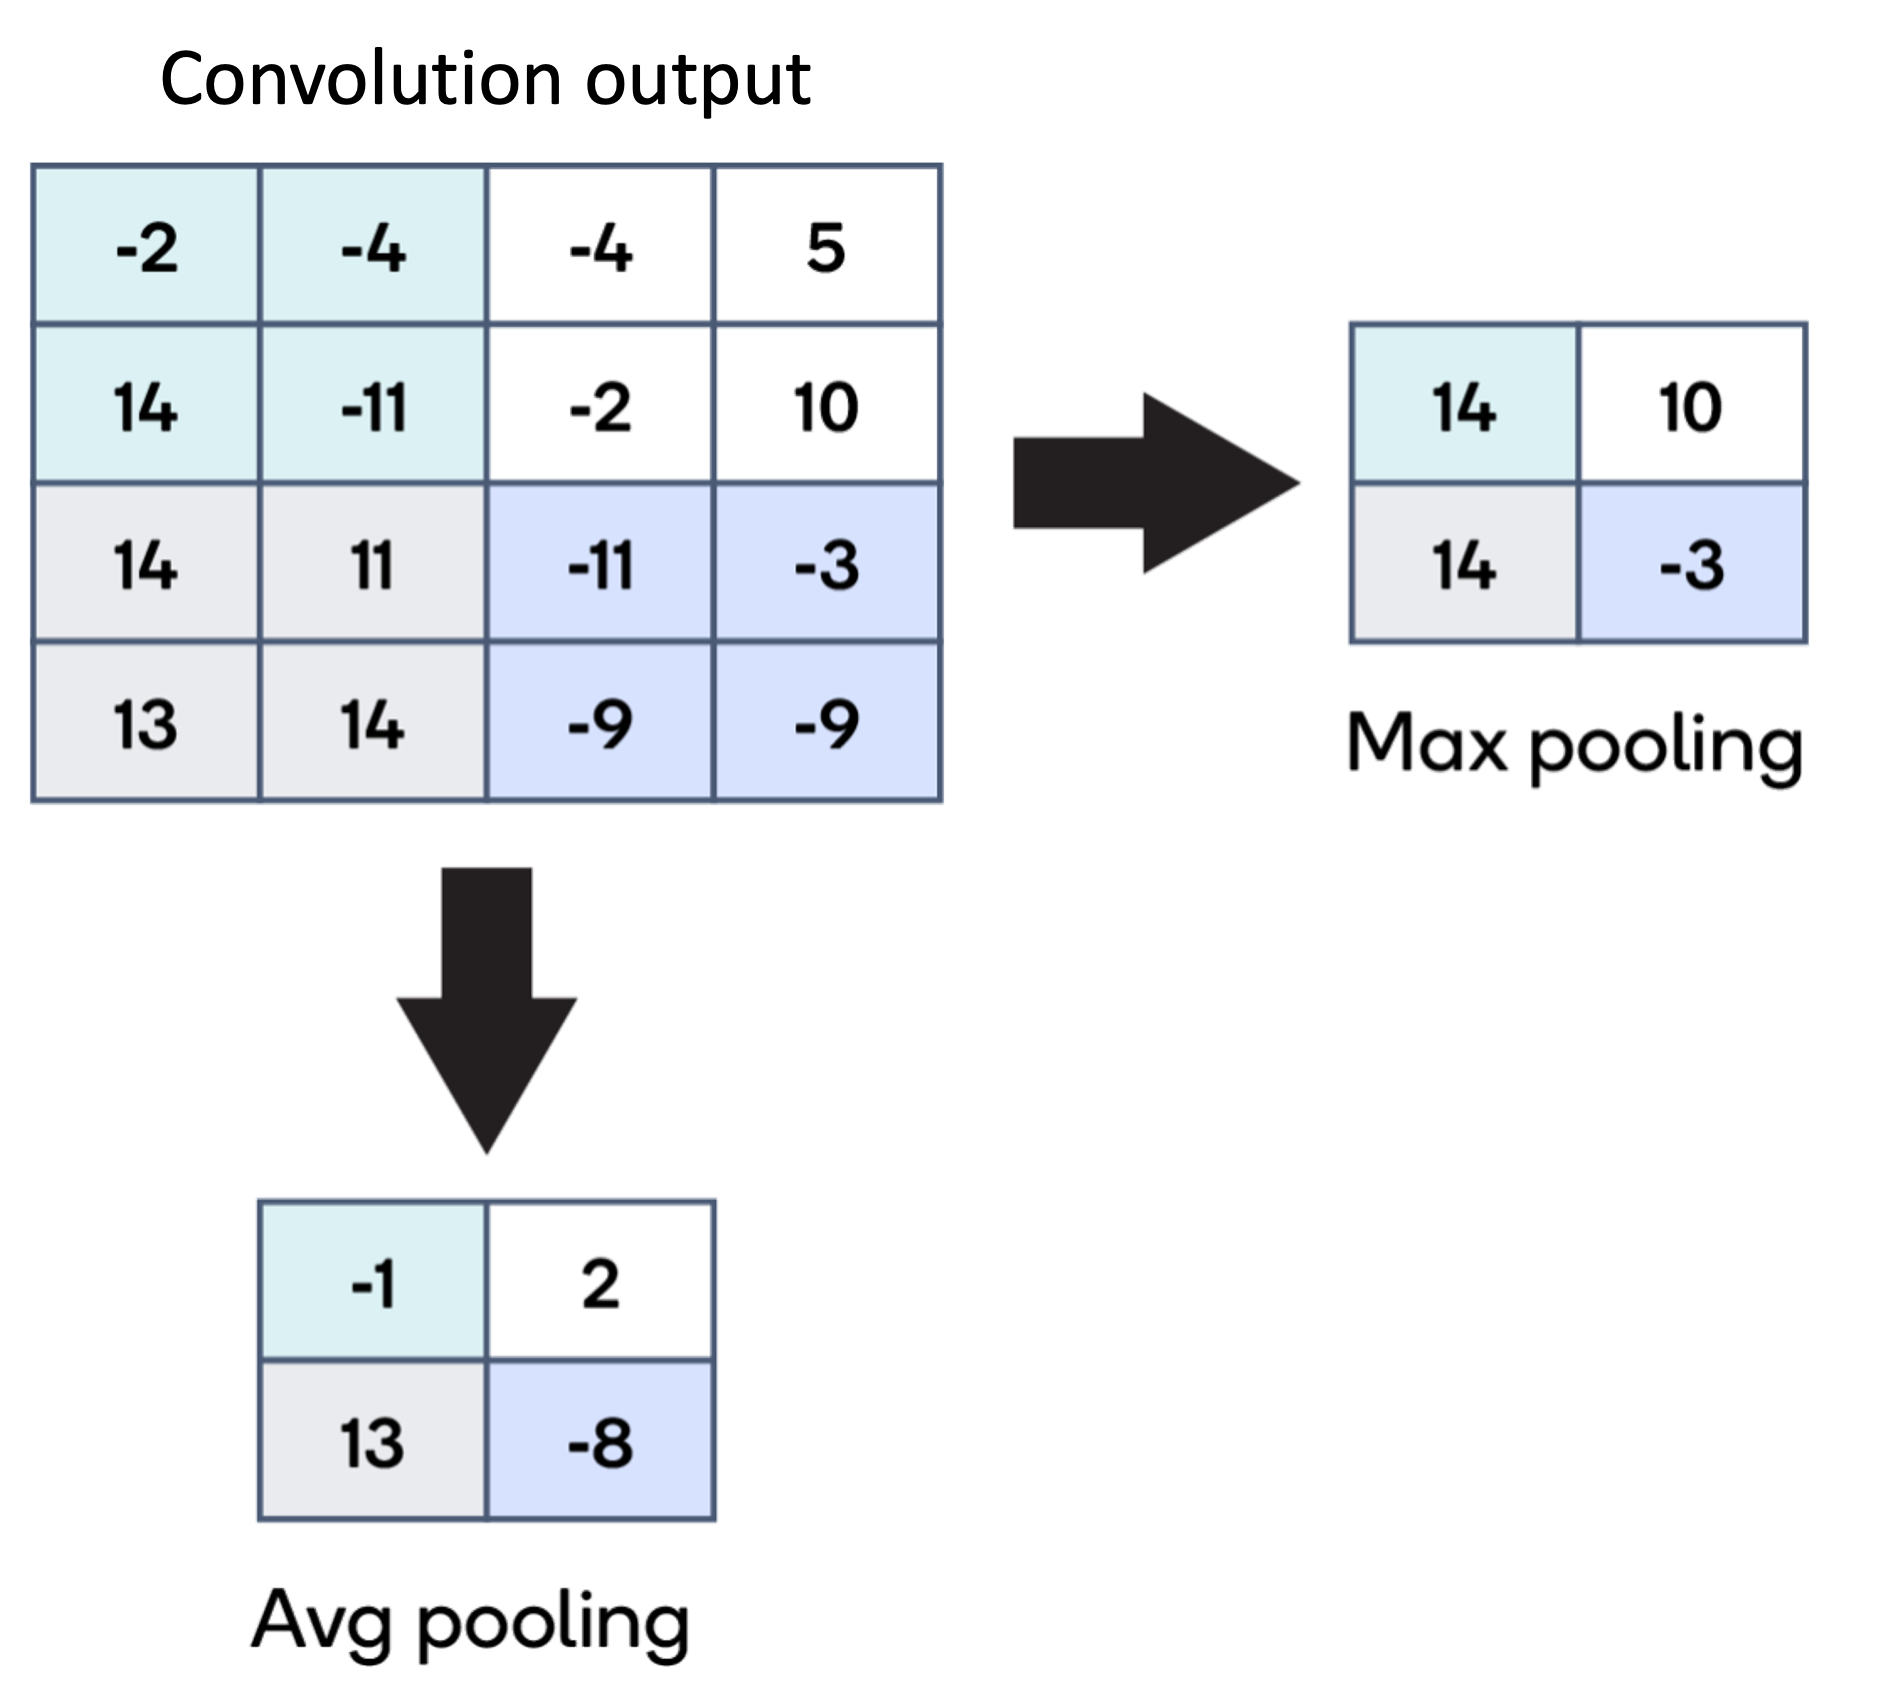
\includegraphics[width=.65\textwidth]{img/pooling.png}
    \end{figure}

    \end{columns}

Uma CNN possui as seguintes camadas\footnote{\tiny{Imagens retiradas de https://www.ibm.com/cloud/learn/convolutional-neural-networks e de https://developer.qualcomm.com/software/qualcomm-neural-processing-sdk/learning-resources/cnn-architectures/deep-learning-convolutional-neural-networks-computer-vision}}:
\begin{itemize}
    \item \textit{\textbf{Convolutional layer}}---serve como um filtro que é usado para extrair as \textit{features} mais importantes do elemento.
    \pause
    \item \textit{\textbf{Pooling layer}}---serve como um filtro para reduzir a dimensionalidade do problema.
\end{itemize}

%% Notes:
\note{-- As an example, let’s assume that we’re trying to determine if an image contains a bicycle. You can think of the bicycle as a sum of parts. It is comprised of a frame, handlebars, wheels, pedals, et cetera. Each individual part of the bicycle makes up a lower-level pattern in the neural net, and the combination of its parts represents a higher-level pattern, creating a feature hierarchy within the CNN.}

\end{frame}
% #############################################################################

% #############################################################################
\begin{frame}{CNNs \cont}

    Uma CNN possui as seguintes camadas:
    \begin{itemize}
    \item \textit{\textbf{Fully-connected layer}}---rede neuronal completamente conectada. É a responsável pela classificação.
\end{itemize}

\pauseskip

Actualmente, existem \textbf{arquitecturas de redes CNN já optimizadas e prontas para serem utilizadas}. As mais conhecidas: AlexNet, GoogLeNet e ResNet.

\pause

\alertbf{Arquitectura da AlexNet:}

\begin{figure}
        \centering
    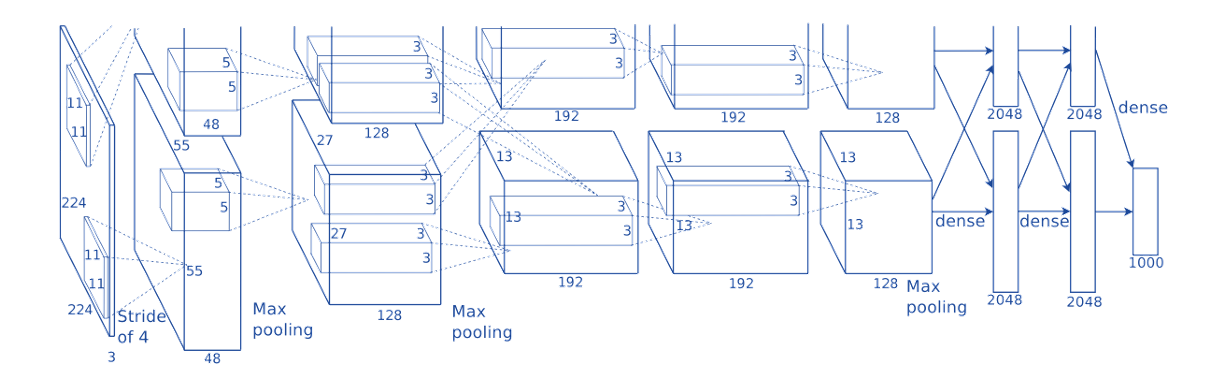
\includegraphics[width=.5\textwidth]{img/alexnet.png}
\end{figure}

Possui cinco \textit{convolutional layers} (algumas delas seguidas por uma \textit{max-pooling layer}) e uma rede neuronal de três camadas.

\end{frame}
% #############################################################################

% #############################################################################
\section{Outros Tipos de Aprendizagem}
% #############################################################################

% #############################################################################
\begin{frame}{\textit{Unsupervised Learning}}

Anteriormente, \textbf{disponibilizámos à rede exemplos de mapeamento entre as entradas e as saídas}. 

\pauseskip

No caso do \textbf{\textit{unsupervised learning}}, esse mapeamento \textbf{não é fornecido à rede}. A rede é, assim, obrigada \textbf{a aprender a classificar os dados com base nos padrões ou nos \textit{clusters}} que encontrar.

\pauseskip

Exemplos de tarefas com \textit{unsupervised learning}:
\begin{itemize}
    \item \textbf{\textit{Clustering}:} quando os dados são agrupados com base na sua semelhança. Por exemplo, as redes \textit{self-organizing map} e $k$-\textit{means clustering}.
    \item \textbf{Redução de dimensionalidade:} quando, de todas as características dos dados, apenas são mantidas algumas. Por exemplo, \textit{autoencoder} e \textit{principal component analysis}.
\end{itemize}

%% Notes:
\note{As self-organizing map aprendem a reconhecer grupos de valores de entradas, de forma a que os neurónios que estiverem mais próximos correspondem a entradas semelhantes.

Um autoencoder é uma rede neural que aprende a copiar sua entrada para sua saída. Possui uma camada interna (oculta) que descreve um código usado para representar a entrada e é constituído por duas partes principais: um codificador que mapeia a entrada no código e um decodificador que mapeia o código para uma reconstrução da entrada. A parte do meio é uma representação reduzida de todas as características da base de dados.
}

\end{frame}
% #############################################################################

% #############################################################################
\begin{frame}{\textit{Reinforcement Learning}}

Neste paradigma, existe um \textbf{agente que autonomamente aprende a tomar decisões, através de tentativa e erro.}

\pauseskip

O agente observa o estado actual do ambiente. Com base nessa observação, \textbf{selecciona uma acção} das várias possíveis. Ao executar a acção, o \textbf{ambiente muda} para um novo estado e o \textbf{agente recebe uma recompensa}, que avalia a eficácia da acção. Esta recompensa, juntamente com o novo estado do ambiente, são enviados para o agente para que este decida a próxima acção a tomar.

\pauseskip

O objectivo do agente é o de \textbf{aprender uma política} (\textit{i.e.}, um conjunto de ações) que leve à \textbf{maximização das recompensas}.

\end{frame}

% #############################################################################
\begin{frame}{\textit{Reinforcement Learning} \cont}

Geralmente, \textbf{os conjuntos de dados são dinamicamente gerados pela interacção do agente com o ambiente}, não sendo, por isso, conjuntos de dados estáticos pré-definidos (tal como nos paradigmas de \textit{supervised} e \textit{unsupervised learning}).

\pauseskip

Um dos mais conhecidos algoritmos de \textit{reinforcement learning} é o $q$-\textit{learning}, onde um \textbf{agente aprende a tomar decisões óptimas explorando} um ambiente e actualizando uma tabela de valores ($q$-\textit{table}) que indicam a qualidade de cada acção em diferentes estados, com base nas \textbf{recompensas recebidas e nas expectativas de recompensas futuras}.

\pauseskip

\textbf{Exemplos de aplicações:} jogos e robótica.

\end{frame}

% #############################################################################

% #############################################################################
\section{\textit{Pipeline} Geral}
% #############################################################################

% #############################################################################
\begin{frame}{\textit{Pipeline} Geral}
    
    \begin{figure}
        \centering
        \resizebox{\textwidth}{!}{
            \begin{tikzpicture}[node distance=2cm]
    \node (data) at (0,0) [process] {Obter dados};
    \node (preprocessing) [process, right of=data, xshift=2cm, align=center] {Pré-processamento \\ de dados};
    \node (preparation) [process, right of=preprocessing, xshift=2cm, align=center] {Preparação \\ de dados};
    \node (init) [process_important, right of=preparation, xshift=2cm, align=center] {Inicialização do \\ modelo};
    \node (train) [process_important, below of=init, align=center] {Treino do \\ modelo};
    \node (evaluate) [process_important, left of=train, xshift=-2cm,align=center] {Avaliação/validação\\ do modelo};
    \node (hyper) [process_important, left of=evaluate,xshift=-2cm,align=center] {Ajuste de\\ hiperparâmetros};
    \node (deploy) [process, left of=hyper, xshift=-2cm,align=center] {Utilização do\\ modelo};
    \draw [arrow] (data) -- (preprocessing);
    \draw [arrow] (preprocessing) -- (preparation);
    \draw [arrow] (preparation) -- (init);
    \draw [arrow] (init) -- (train);
    \draw [arrow] (train) -- (evaluate);
    \draw [arrow] (evaluate) -- (hyper);
    \draw [arrow] (hyper) -- (deploy);
    \draw [arrow] (hyper) |- + (0,-1) -| + (10,2) -- (init);
  \end{tikzpicture}
        }
    \end{figure}

\end{frame}
% #############################################################################

% #############################################################################
\section{Considerações Éticas em IA}
% #############################################################################


% #############################################################################
\begin{frame}{Considerações Éticas em IA}
    
    \begin{columns}
    \begin{column}{0.45\textwidth}
        \metroset{block=fill}
        \begin{alertblock}{\textit{Bias}}
            Consiste na incorporação de decisões humanas tendenciosas ou desigualdades históricas e sociais em sistemas de IA.
        \end{alertblock}
    \end{column}
    \pause
    \begin{column}{0.45\textwidth}
        \metroset{block=fill}
        \begin{alertblock}{\textit{Fairness}}
            Garante que os sistemas de IA são avaliados de forma justa, sem favorecer ou prejudicar injustamente qualquer grupo num conjunto de dados.
        \end{alertblock}
    \end{column}
\end{columns}

\pauseskip

\alertbf{IA Explicável (Explainable AI--XAI)}

Conjunto de métodos que permite aos utilizadores \textbf{entenderem as respostas que são dadas pelos sistemas de AI}, aumentando, desta forma, a confiança, a transparência e facilitando a identificação e a correcção de \textit{bias}.

\end{frame}
% #############################################################################